\documentclass[10pt]{article}\usepackage[]{graphicx}\usepackage[]{color}
% maxwidth is the original width if it is less than linewidth
% otherwise use linewidth (to make sure the graphics do not exceed the margin)
\makeatletter
\def\maxwidth{ %
  \ifdim\Gin@nat@width>\linewidth
    \linewidth
  \else
    \Gin@nat@width
  \fi
}
\makeatother

\definecolor{fgcolor}{rgb}{0.345, 0.345, 0.345}
\newcommand{\hlnum}[1]{\textcolor[rgb]{0.686,0.059,0.569}{#1}}%
\newcommand{\hlstr}[1]{\textcolor[rgb]{0.192,0.494,0.8}{#1}}%
\newcommand{\hlcom}[1]{\textcolor[rgb]{0.678,0.584,0.686}{\textit{#1}}}%
\newcommand{\hlopt}[1]{\textcolor[rgb]{0,0,0}{#1}}%
\newcommand{\hlstd}[1]{\textcolor[rgb]{0.345,0.345,0.345}{#1}}%
\newcommand{\hlkwa}[1]{\textcolor[rgb]{0.161,0.373,0.58}{\textbf{#1}}}%
\newcommand{\hlkwb}[1]{\textcolor[rgb]{0.69,0.353,0.396}{#1}}%
\newcommand{\hlkwc}[1]{\textcolor[rgb]{0.333,0.667,0.333}{#1}}%
\newcommand{\hlkwd}[1]{\textcolor[rgb]{0.737,0.353,0.396}{\textbf{#1}}}%
\let\hlipl\hlkwb

\usepackage{framed}
\makeatletter
\newenvironment{kframe}{%
 \def\at@end@of@kframe{}%
 \ifinner\ifhmode%
  \def\at@end@of@kframe{\end{minipage}}%
  \begin{minipage}{\columnwidth}%
 \fi\fi%
 \def\FrameCommand##1{\hskip\@totalleftmargin \hskip-\fboxsep
 \colorbox{shadecolor}{##1}\hskip-\fboxsep
     % There is no \\@totalrightmargin, so:
     \hskip-\linewidth \hskip-\@totalleftmargin \hskip\columnwidth}%
 \MakeFramed {\advance\hsize-\width
   \@totalleftmargin\z@ \linewidth\hsize
   \@setminipage}}%
 {\par\unskip\endMakeFramed%
 \at@end@of@kframe}
\makeatother

\definecolor{shadecolor}{rgb}{.97, .97, .97}
\definecolor{messagecolor}{rgb}{0, 0, 0}
\definecolor{warningcolor}{rgb}{1, 0, 1}
\definecolor{errorcolor}{rgb}{1, 0, 0}
\newenvironment{knitrout}{}{} % an empty environment to be redefined in TeX

\usepackage{alltt}
\usepackage{graphicx, verbatim}
\usepackage[utf8]{inputenc}
\usepackage{amsmath}
\usepackage{amssymb}
\usepackage{amscd}
\usepackage{lipsum}
\usepackage{blindtext}
\usepackage{todonotes}
\usepackage[tableposition=top]{caption}
\usepackage{ifthen}
\usepackage{caption}
\setlength{\textwidth}{6.5in} 
\setlength{\textheight}{9in}
\setlength{\oddsidemargin}{0in} 
\setlength{\evensidemargin}{0in}
\setlength{\topmargin}{-1.5cm}
\setlength{\parindent}{0cm}
\usepackage{setspace}
\usepackage{float}
\usepackage{fancyhdr}
\usepackage{tabularx}
\usepackage{soul} 

\usepackage{hyperref}
\hypersetup{
  colorlinks   = true, %Colours links instead of ugly boxes
  urlcolor     = blue, %Colour for external hyperlinks
  linkcolor    = blue, %Colour of internal links
  citecolor   = red %Colour of citations
}

\usepackage[backend=biber ,sorting=none]{biblatex}
\bibliography{references}
\begin{filecontents*}{references.bib}
\end{filecontents*}


%\fancyhf{}
\rfoot{Group 2 \thepage}
\singlespacing
\usepackage[affil-it]{authblk} 
\usepackage{etoolbox}
\usepackage{lmodern}

% \makeatletter
% \renewcommand{\maketitle}{\bgroup\setlength{\parindent}{16pt}
% \begin{flushleft}
%   \textbf{\@title}
% 
%   \@author
% \end{flushleft}\egroup
% }

%\renewcommand\Authfont{\fontsize{14}{18.4}\selectfont}
%\makeatother

% \pagestyle{fancy}
% \rfoot{Page \thepage}
 %\thispagestyle{empty} 



\IfFileExists{upquote.sty}{\usepackage{upquote}}{}
\begin{document}

\title{\LARGE Professional Development and Research Skills \\ CMM507 Coursework  \\ Group 2: Plastic Pollution in Oceans}

\author{ALEXANDER RITCHIE, \textit{\href{1911218@rgu.ac.uk}{1911218@rgu.ac.uk}};\\ GEORGIOS ORFANAKIS, \textit{\href{1903446@rgu.ac.uk}{1903446@rgu.ac.uk}};\\ KAREN JEWELL, \textit{\href{1415410@rgu.ac.uk}{1415410@rgu.ac.uk}};\\ ROSHI SHRESTHA, \textit{\href{1903445@rgu.ac.uk}{1903445@rgu.ac.uk}};\\ STUART WATT, \textit{\href{1501869@rgu.ac.uk}{1501869@rgu.ac.uk}}}

\maketitle
\noindent\rule{16cm}{0.4pt}


\section{Problem Statement}

\subsection{Overview}\label{over}

Marine pollution is a major global issue which impacts the environment, economy and human health. Although marine pollution is caused by many different materials, plastics consist of 60-80\% of the marine litter. \cite{DERRAIK2002} \cite{SMITH2013} \cite{KUO2014} \cite{ZHOU2011} \cite{JANG2014} Plastics are synthetic organic polymers and their lightweight feature and durability make it very suitable to make a range of products we use in our everyday life.\cite{BARNES2009} \cite{SIVAN2011} These same features are what makes plastic a major component of pollution, due to overuse and non-managed waste disposal systems internationally, contributing to 10\% of the waste generated worldwide.\cite{BARNES2009} As the global production of plastic increases, so does the problem in the marine environment. Due to its buoyancy, plastic debris can be dispersed over long distances and accumulate on the shorelines, even polluting the most remote areas \cite{LAVERS2017}. Jambeck et al.,\cite{JAMBECK2015} reported that in 2010 alone, between 4.8 million and 12.7 million metric tons of plastics entered the ocean. Plastics are everywhere in the marine environment and urgent action is required to mitigate this problem and reduce its harmful impact.\cite{RIOS2007} \cite{ROCHMAN2015} \\



\subsection{Motivation}\label{mot}

The impact of plastic pollution on marine life has been reviewed extensively. \cite{GALL2015} \cite{KUHN2015} \cite{RYAN2015} \cite{WILLIAMS2019} Over 700 marine wildlife species are affected due to entanglement in plastic ropes or materials, and from ingestion of plastics in the ocean.\cite{GALL2015} Over time, plastic disintegrates into microplastics and nanoplastics which are easily consumed by fish and enter the human food chain. Plastics have been found in a third of fish caught in the UK which included popular fish such as cod, haddock, and mackerel.\cite{LUSHER2013} The impact and effects of plastic entering the human food chain are still being studied, but plastic toxicity and the occurrence of microplastics and nanoplastics in the water supply also directly impacts human health, in addition to the contamination of seafood.\cite{ROCHMAN2015} \cite{MARKIC2020} \\

Although plastic litter has been a major cause of marine pollution for a while, its seriousness has only been realised recently and reducing plastic pollution has become a global aim. Research on plastic pollution in marine environments has played a big role in efforts to reduce it as well as in raising awareness globally. In order to understand plastic pollution in marine environments and its effects in the long term, it is essential to keep collecting data on patterns of marine debris around the world. Effective monitoring of plastic debris is essential to reducing the abundance of plastic debris everywhere. In addition, monitoring the type, frequency and the source of the litter is also important for marine pollution prevention initiatives. Most monitoring is done by survey, where organisations and volunteers record the types and frequencies of litter observed on the shoreline.\cite{COE1997} To understand the depth of the problem, it is essential to understand the amount and composition of marine litter. This can help in applying various mitigation strategies.\\

\subsection{Objectives }\label{obj}

The main objectives of this project is outlined as follows:
\begin{itemize}	
\item To review available literature on marine plastic problems and their impacts
\item To look at a suitable dataset to understand the composition of marine plastic pollution 
\item To create a linear regression model to predict the relevant frequency of distinct plastic debris categories over time
\item To present the derived results and conclusions 

\end{itemize}





























\pagebreak
\section{Research}\label{research}

An integral part of this report required a literature search to identify how researchers have been trying to monitor marine pollution and find the problems associated with it. Several studies have reported the abundance of plastic as marine litter through scientific survey and citizen science methods. A 12-year observation of coastal debris pollution using citizen science in Taiwan revealed that most debris items found were plastic. \cite{WALTHER2018} 19 categories of debris items were collected during the clean-up events and the five most commonly recorded debris categories were: plastic shopping bags, plastic bottle caps, disposable tablewares, fishing equipment, and plastic drinking straws. In a study covering western Japan and the eastern coasts of Russia \cite{KUSUI2003}, it found that 55\% to 93.4\% of items over the Japanese shores were plastic, and the second most abundant item was resin pellet which is also a form of plastic. On the eastern Russian coast, plastic items were also the most abundant, contributing to approximately 55\% of all litter, mostly of plastic fragments. The composition of litter was similar in the two countries, although the proportion of plastics was much higher in Japan. \cite{KUSUI2003} Further along the Asian upper east coast, hard plastic and styrofoam were the dominant plastic types found on Korean beaches. On average, hard plastic and styrofoam comprised 32\% and 48.5\% of the total debris count respectively. \\

In an older study over the Caribbean region, the most common types of debris found on the Caribbean coast of Panama were plastic and styrofoam, with the plastics being household or consumer related. Styrofoam packing materials were also abundant and may have come from trans-shipment activities of Colon's Free Zone, household waste, or offshore activity \cite{GARRITY1993}. A 2016/2017 annual study of 8 beaches in Tenerife in the Canary Islands also found that plastic was the most abundant litter there. They also reported that there was more accumulated plastic debris in remote beaches compared to the beaches near the city indicating the movement of debris. However, more long term study is required to understand the changes in the results reported over time. \cite{REINOLD2020} \\

It was observed by the authors of this report, that there were variations in how studies of litter accumulation had been conducted. The variations are present in the time span of the research, the parts of the coast from which litter was collected, as well as in the categorisation of litter, which creates difficulty when researchers want to compare different studies. The plastic pollution problem essentially requires the ability to assess changes in accumulation rates and composition, trends over time, and the effectiveness of management systems, which is a hard task without good monitoring methodologies. Although monitoring of marine litter is currently carried out within a number of countries around the world, the methods of survey and monitoring used tend to be very different, preventing comparisons and harmonisation of data across regions or time. \\

This is why the scientific community has been trying to create some common ground, which has led to initiatives joined by many countries worldwide. One of these initiatives, and probably the most important, is the International Clean Coast (ICC) program which is a new, long term approach to cleaner beaches using various activities to increase public awareness. \cite{ CHESHIRE2009} This initiative aims to develop a comprehensive litter characterisation scheme that uses both material composition and form. This allows Litter Monitoring Repeated (LMR) surveys of beaches, seabeds and/or surface waters to determine litter quantities such that information can be compared with baseline data to identify if changes occur over time or in response to management arrangements. \\

The ICC uses specifically developed categorisations of coast litter, with the most accepted being the Clean Coastal Index (CCI) protocol specific to the operational clean-up of beaches, which is useful for its simplicity and information provided, allowing comparisons between different times and places. The CCI is the recommended tool for evaluation of actual coast cleanliness, measuring plastic debris as an indicator of beach cleanliness, precluding bias by the assessor. The CCI also proved to be a useful tool for measuring progress and the success of activities in raising awareness among the general public. \cite{ALKALAY2007} \\

A study in Israel using the CCI protocol for categorisation found that plastic was the most ubiquitous beach litter item. An important contribution to this study was the ability to compare its findings to other Mediterranean beaches, showing that plastic was the dominant pollutant in the region, and non-plastic litter being highly specific to the region and cannot be treated universally. \cite{PORTMAN2017} In another study on litter pollution in a region of India, once again following the CCI protocol for the categorisation of litter, found that plastic was the main form of litter at approximately 45\% of total litter. Plastic bags topped the index at 33\%, followed by food wrappers, then plastic cups, and cigarette/cigar tips amounting to 5.5\%. \cite{KUMAR2016} The use of the common protocol in these two studies allowed researchers to compare their findings and create common plastic pollution models, even though the two coasts are continents apart. \\

Another study conducted in Cadiz, on the other side of the Mediterranean from Israel, found that plastic bottles and containers were the most frequent littered items, followed by plastic bags. This research also pointed out that surveys are heavily affected by clean-ups performed at beaches. \cite{WILLIAMS2016} Even though this study reaches important conclusions on the correct ways to clean coasts, it cannot be easily compared, or its conclusions easily applied without any standardised protocol. \\

From this review, it is evident that there have been many studies conducted to monitor marine pollution in various different ways. One of the most cost effective and efficient ways is the use of citizen science, where the general public can record any observations of marine litter \cite{EARP2019} and has beens been successfully used in many studies. \cite{ROY2012} \cite{FORRESTER2015} This method is also gaining popularity in marine pollution monitoring \cite{BRAVO2009} \cite{CARSON2012} \cite{HIDALGORUZ2017} \cite{BAUERCIVIELLO2018} and has also been assessed as a tool to increase awareness of the marine litter problem. \cite{LOCRITANI2019} \\


As discussed before, observations not following a standard protocol with proper guidance could be incomparable and rendered ineffective. The Marine Debris Tracker (MDT) is a joint initiative between National Oceanic and Atmospheric Administration (NOAA) Marine Debris Program (MDP) and the Universities of Georgia, North Carolina and South Carolina \cite{JAMBECK2015B}. The MDT allows anyone to record the marine debris observed, using an application on a mobile phone. The only report using data from this application is a web-based report by Tablada in 2018 \cite{JAMBECK2015B}, where data analysis was performed on 8 years of the data mainly focused in North America. The study also concluded that plastic was the main type of debris recorded, with cigarettes being the top identified littered item. The subsequent sections of this report will aim to contribute to this body of knowledge, using the worldwide coastal littering dataset from the MDT, with an interest in identifying if plastic is indeed the most abundant litter of the worldwide dataset, which would be in agreement with the various studies discussed in this review. Following which, this report will analyse the distribution of subclasses within the plastics found, and explore if there could be a way to computationally monitor and assess the coastal littering problem, using the established CCI categorisation of litter. \\








\pagebreak
\section {Methods}\label{methods}

\subsection{Data Description}\label{dataset}

The data used in this report was gathered using secondary data collection methods only. The authors did not collect or create any new data using primary methods. The data was downloaded from the Marine Debris Tracker website (\url{www.marinedebris.engr.uga.edu}) on \hl{what was the date of download?}. The dataset is composed of 363,368 global observations from the start of the program in 2010, to the latest available date at the time of download. \\

As discussed in the section before, the MDT is a citizen science project where organisations or individuals can record observations of marine debris using a mobile phone application. \cite{JAMBECK2015B} The user records the observation using a structured form, and chooses the category of debris from a list provided but there are also multiple available fields to populate, including non-mandatory fields and some allowing free text entry. An example of a non-mandatory field are "Lists" which are customisable groupings usually for organisations to group their own collection of records.The table below describes the structure of the data. 

\begin{table}[H]
\begin{tabular}{ l l l }
Field & Description & Type \\
\hline
ListName & custom groupings of records & Non-mandatory \\
ListID & ID for ListName & Automated \\
ItemName & the category of debris & Mandatory \\
ItemID & ID for ItemName & Automated \\
LogID & unique ID for the observation & Automated \\
Quantity & the number of pieces of debris observed & Mandatory \\
Error radius & radius around the site within the error for reasonable doubt & Mandatory \\
Latitude & coordinates of the location where the observation was made & Mandatory \\
Longitude & coordinates of the location where the observation was made & Mandatory \\
Altitude & coordinates of the location where the observation was made & Mandatory \\
Location & text description of the location where the observation was made & Mandatory \\
Description & open text description for the observation & Non-mandatory \\
MaterialDescription & the material of the debris & Mandatory \\
MaterialID & ID for MaterialDescription & Automated \\
Timestamp & the date and time of observation & Mandatory \\
\end{tabular}
\end{table}



\pagebreak
\subsection{Data Pre-processing}\label{preprocessing}

\begin{knitrout}\small
\definecolor{shadecolor}{rgb}{0.969, 0.969, 0.969}\color{fgcolor}\begin{kframe}
\begin{alltt}
\hlcom{# Setting the environment}
\hlkwd{library}\hlstd{(tidyverse)}
\hlkwd{library}\hlstd{(purrr)}
\hlkwd{library}\hlstd{(magrittr)}
\hlkwd{library}\hlstd{(treemap)}
\hlkwd{library}\hlstd{(hexbin)}
\hlkwd{library}\hlstd{(mapdata)}
\hlkwd{library}\hlstd{(viridis)}
\hlkwd{library}\hlstd{(lubridate)}
\hlkwd{library}\hlstd{(imager)}
\hlkwd{library}\hlstd{(xtable)}
\hlkwd{library}\hlstd{(dplyr)}

\hlcom{# Loading the data}
\hlstd{data} \hlkwb{<-} \hlkwd{list.files}\hlstd{(}\hlkwc{path} \hlstd{=} \hlstr{"data/debris/"}\hlstd{,} \hlkwc{full.names} \hlstd{=} \hlnum{TRUE}\hlstd{)} \hlopt
  \hlkwd{lapply}\hlstd{(}\hlkwc{FUN} \hlstd{= read_csv,} \hlkwc{col_types} \hlstd{=} \hlstr{"ififidddddcfcif"}\hlstd{)} \hlopt
  \hlkwd{reduce}\hlstd{(rbind)}

\hlcom{# Checking the size of the data}
\hlkwd{cat}\hlstd{(}\hlstr{"rows: "}\hlstd{,} \hlkwd{nrow}\hlstd{(data),}\hlstr{"; columns: "}\hlstd{,} \hlkwd{ncol}\hlstd{(data))}
\end{alltt}
\begin{verbatim}
## rows:  363368 ; columns:  15
\end{verbatim}
\end{kframe}
\end{knitrout}



From download, the data was cleaned to prepare it for analysis. First, the \textbf{Timestamp} datetime information was converted into a date type format and renamed as variable \textbf{Time}

\begin{knitrout}\small
\definecolor{shadecolor}{rgb}{0.969, 0.969, 0.969}\color{fgcolor}\begin{kframe}
\begin{alltt}
\hlcom{# Replacing the column for time as a date data type, renaming it "Time" }
\hlstd{data}\hlopt{$}\hlstd{Time} \hlkwb{<-} \hlstd{data}\hlopt{$}\hlstd{Timestamp} \hlopt
  \hlkwd{parse_datetime}\hlstd{(}\hlkwc{format} \hlstd{=} \hlstr{"%Y%m%d%H%M%S"}\hlstd{)}
\hlstd{data}\hlopt{$}\hlstd{Timestamp} \hlkwb{<-} \hlkwa{NULL}
\end{alltt}
\end{kframe}
\end{knitrout}


The dataset was then inspected for missing values which were observed in the \textbf{Location} and \textbf{Description} fields, but as these are non-mandatory and open text fields it is to be expected, and all other fields are complete.\\ 
\begin{knitrout}\small
\definecolor{shadecolor}{rgb}{0.969, 0.969, 0.969}\color{fgcolor}\begin{kframe}
\begin{alltt}
\hlcom{# Identifying missing values}
\hlstd{data} \hlopt \hlkwd{select_if}\hlstd{(}\hlkwa{function}\hlstd{(}\hlkwc{x}\hlstd{)} \hlkwd{any}\hlstd{(}\hlkwd{is.na}\hlstd{(x)))} \hlopt \hlkwd{colnames}\hlstd{()}
\end{alltt}
\begin{verbatim}
## [1] "Location"    "Description"
\end{verbatim}
\end{kframe}
\end{knitrout}

It was observed that observations were incomplete for years 2010, 2011 and 2020, and so it was decided to retain only complete years of information for fair and standard comparisons.
\begin{knitrout}\small
\definecolor{shadecolor}{rgb}{0.969, 0.969, 0.969}\color{fgcolor}\begin{kframe}
\begin{alltt}
\hlcom{# Count the number of months in each year}
\hlstd{data} \hlopt
  \hlkwd{mutate}\hlstd{(}\hlkwc{year} \hlstd{=} \hlkwd{year}\hlstd{(Time),}
         \hlkwc{months} \hlstd{=} \hlkwd{month}\hlstd{(Time))} \hlopt
  \hlkwd{select}\hlstd{(year, months)} \hlopt
  \hlkwd{unique}\hlstd{()} \hlopt
  \hlkwd{group_by}\hlstd{(year)} \hlopt
  \hlkwd{summarize}\hlstd{(}\hlkwc{nmonths} \hlstd{=} \hlkwd{n}\hlstd{())}
\end{alltt}
\begin{verbatim}
## # A tibble: 11 x 2
##     year nmonths
##    <dbl>   <int>
##  1  2010       1
##  2  2011      10
##  3  2012      12
##  4  2013      12
##  5  2014      12
##  6  2015      12
##  7  2016      12
##  8  2017      12
##  9  2018      12
## 10  2019      12
## 11  2020       2
\end{verbatim}
\end{kframe}
\end{knitrout}

\begin{knitrout}\small
\definecolor{shadecolor}{rgb}{0.969, 0.969, 0.969}\color{fgcolor}\begin{kframe}
\begin{alltt}
\hlcom{# Filter for observations occuring between the years 2012-2019 inclusive}
\hlstd{data} \hlkwb{<-} \hlstd{data} \hlopt \hlkwd{filter}\hlstd{(}\hlkwd{as.integer}\hlstd{(}\hlkwd{year}\hlstd{(Time))} \hlopt \hlnum{2012}\hlopt{:}\hlnum{2019}\hlstd{)}
\end{alltt}
\end{kframe}
\end{knitrout}

\begin{knitrout}\small
\definecolor{shadecolor}{rgb}{0.969, 0.969, 0.969}\color{fgcolor}\begin{kframe}
\begin{alltt}
\hlcom{# Checking the size of the data}
\hlkwd{cat}\hlstd{(}\hlstr{"rows: "}\hlstd{,} \hlkwd{nrow}\hlstd{(data),}\hlstr{"; columns: "}\hlstd{,} \hlkwd{ncol}\hlstd{(data))}
\end{alltt}
\begin{verbatim}
## rows:  349556 ; columns:  15
\end{verbatim}
\end{kframe}
\end{knitrout}

Assessing the dataset for unique items it was observed that there are 8 material categories containing 55 different item subcategories and with them 7982 unique descriptions across the 349,556 observations. 
\begin{kframe}
\begin{alltt}
\hlcom{# Counting unique values in fields}
\hlstd{data} \hlopt
  \hlkwd{summarise_all}\hlstd{(}\hlopt{~}\hlkwd{length}\hlstd{(}\hlkwd{unique}\hlstd{(.)))} \hlopt
  \hlkwd{pivot_longer}\hlstd{(}\hlkwc{cols} \hlstd{=} \hlkwd{everything}\hlstd{(),}
               \hlkwc{names_to} \hlstd{=} \hlstr{"Field"}\hlstd{,}
               \hlkwc{values_to} \hlstd{=} \hlstr{"Unique Values"}\hlstd{)} \hlopt
  \hlkwd{arrange}\hlstd{(}\hlkwd{desc}\hlstd{(`Unique Values`))} \hlopt
  \hlkwd{xtable}\hlstd{(}\hlkwc{caption} \hlstd{=} \hlstr{"The count of unique values in fields"}\hlstd{,}
         \hlkwc{label} \hlstd{=} \hlstr{"tab:unique"}\hlstd{,}
         \hlkwc{caption.placement} \hlstd{=} \hlstr{"top"}\hlstd{,}
         \hlkwc{floating}\hlstd{=}\hlnum{TRUE}\hlstd{,}
         \hlkwc{type}\hlstd{=}\hlstr{"latex"}\hlstd{,}
         \hlkwc{table.placement} \hlstd{=} \hlstr{"H"}\hlstd{)}
\end{alltt}
\end{kframe}% latex table generated in R 3.6.1 by xtable 1.8-4 package
% Mon May 11 11:58:33 2020
\begin{table}[ht]
\centering
\begin{tabular}{rlr}
  \hline
 & Field & Unique Values \\ 
  \hline
1 & LogID & 349556 \\ 
  2 & Time & 237066 \\ 
  3 & Latitude & 144820 \\ 
  4 & Altitude & 133174 \\ 
  5 & Longitude & 132316 \\ 
  6 & Error Radius & 16930 \\ 
  7 & Description & 7982 \\ 
  8 & Location & 1352 \\ 
  9 & Quantity & 494 \\ 
  10 & ItemID &  55 \\ 
  11 & ItemName &  55 \\ 
  12 & Material ID &   8 \\ 
  13 & Material Description &   8 \\ 
  14 & ListID &   1 \\ 
  15 & ListName &   1 \\ 
   \hline
\end{tabular}
\caption{The count of unique values in fields} 
\label{tab:unique}
\end{table}


It is difficult to determine exactly how many global locations are observed in this dataset as it is the combination of \textbf{Longitude}, \textbf{Latitude}, \textbf{Altitude} and/or \textbf{Location} which determines the global position of the observation. 


\pagebreak
\subsection{Quantities}\label{quantities}

In exploring the dataset, it was noted that there was a highly skewed distribution of \textbf{Quantities} recorded per observation.

\begin{figure}[H] 
\begin{center}
\begin{knitrout}\small
\definecolor{shadecolor}{rgb}{0.969, 0.969, 0.969}\color{fgcolor}\begin{kframe}
\begin{alltt}
\hlcom{# Scatter plot showing distribution of observation quantities}
\hlstd{data} \hlopt
  \hlkwd{mutate}\hlstd{(}\hlkwc{Year} \hlstd{=} \hlkwd{as.integer}\hlstd{(}\hlkwd{year}\hlstd{(Time)))} \hlopt
  \hlkwd{select}\hlstd{(Quantity, Year)} \hlopt
  \hlkwd{group_by}\hlstd{(Quantity, Year)} \hlopt
  \hlkwd{summarise}\hlstd{(}\hlkwc{density} \hlstd{=} \hlkwd{n}\hlstd{())} \hlopt
  \hlkwd{ggplot}\hlstd{(}\hlkwd{aes}\hlstd{(}\hlkwc{x}\hlstd{=Quantity,} \hlkwc{y}\hlstd{=density))} \hlopt{+}
    \hlkwd{geom_point}\hlstd{()} \hlopt{+}
    \hlkwd{scale_x_continuous}\hlstd{(}\hlkwc{trans} \hlstd{=} \hlstr{'log10'}\hlstd{)} \hlopt{+}
    \hlkwd{theme_bw}\hlstd{()} \hlopt{+}
    \hlkwd{theme}\hlstd{(}\hlkwc{panel.grid.major} \hlstd{=} \hlkwd{element_blank}\hlstd{(),}
          \hlkwc{panel.grid.minor} \hlstd{=} \hlkwd{element_blank}\hlstd{())}
\end{alltt}
\end{kframe}
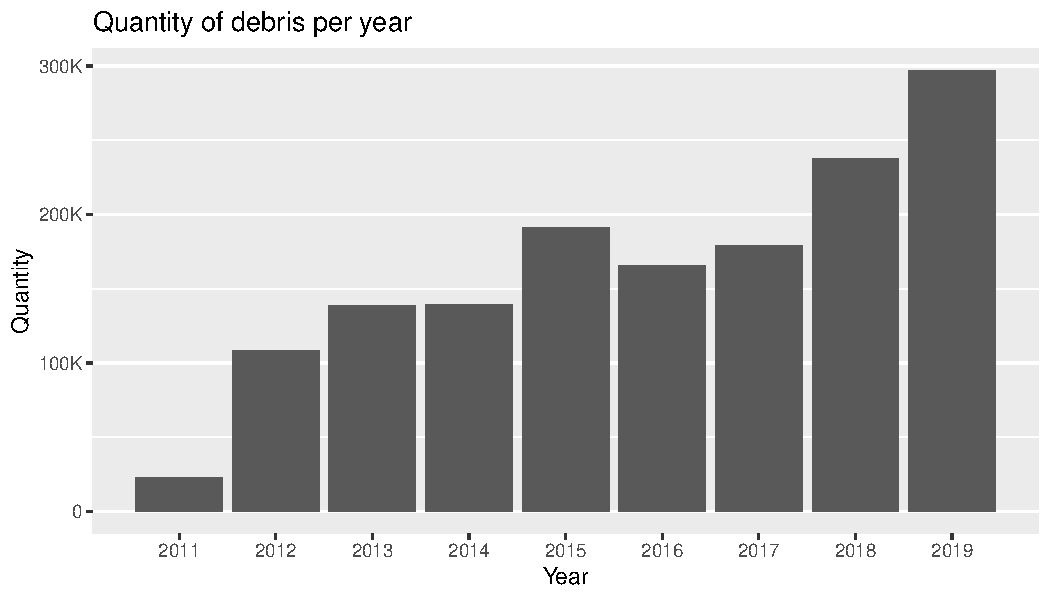
\includegraphics[width=1\linewidth]{figure/unnamed-chunk-9-1} 

\end{knitrout}
\caption {Quantities Distribution}
\label{figE1}
\end {center}
\end {figure}

\begin{kframe}
\begin{alltt}
\hlcom{# Distribution of Quantities}
\hlstd{data} \hlopt
  \hlkwd{select}\hlstd{(Quantity)} \hlopt
  \hlkwd{summary}\hlstd{()}
\end{alltt}
\end{kframe}    Quantity        
 Min.   :     0.00  
 1st Qu.:     1.00  
 Median :     1.00  
 Mean   :     4.17  
 3rd Qu.:     1.00  
 Max.   :100000.00  
\begin{kframe}\begin{alltt}
\hlcom{# Identifying observations with the largest 10 quantities}
\hlstd{data} \hlopt
  \hlkwd{mutate}\hlstd{(}\hlkwc{Year} \hlstd{=} \hlkwd{as.integer}\hlstd{(}\hlkwd{year}\hlstd{(Time)))} \hlopt
  \hlkwd{select}\hlstd{(`Material Description`,ItemName,Year,Description,Quantity)} \hlopt
  \hlkwd{arrange}\hlstd{(}\hlkwd{desc}\hlstd{(Quantity))} \hlopt
  \hlkwd{head}\hlstd{(}\hlnum{10}\hlstd{)}\hlopt
  \hlkwd{xtable}\hlstd{(}\hlkwc{caption} \hlstd{=} \hlstr{"Observations with the 10 largest quantities"}\hlstd{,}
         \hlkwc{label} \hlstd{=} \hlstr{"tab:top10quantities"}\hlstd{,}
         \hlkwc{caption.placement} \hlstd{=} \hlstr{"top"}\hlstd{,}
         \hlkwc{align} \hlstd{=} \hlstr{"lp\{2cm\}p\{2cm\}lp\{7cm\}l"}\hlstd{,}
         \hlkwc{floating}\hlstd{=}\hlnum{TRUE}\hlstd{,}
         \hlkwc{type}\hlstd{=}\hlstr{"latex"}\hlstd{,}
         \hlkwc{table.placement}\hlstd{=}\hlstr{"H"}\hlstd{)}
\end{alltt}
\end{kframe}% latex table generated in R 3.6.1 by xtable 1.8-4 package
% Mon May 11 11:58:38 2020
\begin{table}[ht]
\centering
\begin{tabular}{lp{2cm}p{2cm}lp{7cm}l}
  \hline
 & Material Description & ItemName & Year & Description & Quantity \\ 
  \hline
1 & RUBBER & Tires & 2019 &  & 100000.00 \\ 
  2 & PLASTIC & Cigarettes & 2012 & Picked up during 20 minute beach cleanups over the course of 116 non consecutive cleanups & 38875.00 \\ 
  3 & PLASTIC & Cigarettes & 2013 &  & 15496.00 \\ 
  4 & PLASTIC & Plastic or Foam Fragments & 2015 &  & 13500.00 \\ 
  5 & PLASTIC & Cigarettes & 2015 &  & 12594.00 \\ 
  6 & PLASTIC & Cigarettes & 2014 &  & 8281.00 \\ 
  7 & PLASTIC & Cigarettes & 2015 &  & 5656.00 \\ 
  8 & PLASTIC & Cigarettes & 2014 &  & 5598.00 \\ 
  9 & PLASTIC & Cigarettes & 2014 & Earth and Surf Fest & 5000.00 \\ 
  10 & PLASTIC & Plastic or Foam Fragments & 2019 &  & 5000.00 \\ 
   \hline
\end{tabular}
\caption{Observations with the 10 largest quantities} 
\label{tab:top10quantities}
\end{table}
\begin{kframe}\begin{alltt}
\hlkwd{length}\hlstd{(data}\hlopt{$}\hlstd{Quantity[data}\hlopt{$}\hlstd{Quantity}\hlopt{<=}\hlnum{100}\hlstd{])}\hlopt{/}\hlkwd{length}\hlstd{(data}\hlopt{$}\hlstd{Quantity)}
\end{alltt}
\end{kframe}[1] 0.9967559
\begin{kframe}\begin{alltt}
\hlkwd{length}\hlstd{(data}\hlopt{$}\hlstd{Quantity[data}\hlopt{$}\hlstd{Quantity}\hlopt{<=}\hlnum{10}\hlstd{])}\hlopt{/}\hlkwd{length}\hlstd{(data}\hlopt{$}\hlstd{Quantity)}
\end{alltt}
\end{kframe}[1] 0.9618373
\begin{kframe}\begin{alltt}
\hlkwd{length}\hlstd{(data}\hlopt{$}\hlstd{Quantity[data}\hlopt{$}\hlstd{Quantity}\hlopt{<=}\hlnum{1}\hlstd{])}\hlopt{/}\hlkwd{length}\hlstd{(data}\hlopt{$}\hlstd{Quantity)}
\end{alltt}
\end{kframe}[1] 0.761692


\hl{any ideas how to present the above \% a bit better?} 99.6\% of all entries have observed quantities below 100, 96\% as 10 or fewer and 76\% as 1 item observed, suggesting that the vast majority of entries are citizen science entries. Interestingly some quantities are marked as 0, and there are a few observations with large quantities observed, possibly as a result of organised or research activity. In particular there are 5 observations with quantities of $>10,000$ recorded in 2012, 2013, 2015 and 2019. It was decided not to exclude these high quantity observations as it would exclude a wealth of information gathered by organised groups or studies. Instead for the majority of this report, the count of observations is deemed to be a fairer indicator of density, rather than the quantity which is influenced heavily by the high quantity counts.

\pagebreak
\subsection{Categorisation}

It is worth noting that of the 8 material categories, one is an "Other" category which allows users to categorise an item as such, if it is not appropriate for any other option on the list.

\begin{kframe}
\begin{alltt}
\hlcom{# Listing of material categories}
\hlstd{data} \hlopt \hlkwd{select}\hlstd{(`Material Description`)} \hlopt
  \hlkwd{unique}\hlstd{()} \hlopt
  \hlkwd{arrange}\hlstd{(`Material Description`)} \hlopt
  \hlkwd{xtable}\hlstd{(}\hlkwc{caption} \hlstd{=} \hlstr{"Listing of Material Descriptions"}\hlstd{,}
         \hlkwc{label} \hlstd{=} \hlstr{"tab:materials"}\hlstd{,}
         \hlkwc{caption.placement} \hlstd{=} \hlstr{"top"}\hlstd{,}
         \hlkwc{floating}\hlstd{=}\hlnum{TRUE}\hlstd{,}
         \hlkwc{type}\hlstd{=}\hlstr{"latex"}\hlstd{,}
         \hlkwc{table.placement}\hlstd{=}\hlstr{"H"}\hlstd{)}
\end{alltt}
\end{kframe}% latex table generated in R 3.6.1 by xtable 1.8-4 package
% Mon May 11 11:58:39 2020
\begin{table}[ht]
\centering
\begin{tabular}{rl}
  \hline
 & Material Description \\ 
  \hline
1 & PAPER \& LUMBER \\ 
  2 & PLASTIC \\ 
  3 & METAL \\ 
  4 & CLOTH \\ 
  5 & OTHER ITEMS \\ 
  6 & FISHING GEAR \\ 
  7 & GLASS \\ 
  8 & RUBBER \\ 
   \hline
\end{tabular}
\caption{Listing of Material Descriptions} 
\label{tab:materials}
\end{table}



A data quality check performed on assessing the debris subcategories were unique by material type, highlighted that the subcategory "Rubber Gloves" was associated with two material types, Plastic and Rubber. Yet otherwise, a one to many relationship exists between the parent material type and their item subcategories suggesting the integrity of the data remains intact.

\begin{knitrout}\small
\definecolor{shadecolor}{rgb}{0.969, 0.969, 0.969}\color{fgcolor}\begin{kframe}
\begin{alltt}
\hlcom{# Checking for subcategory uniqueness}
\hlstd{data} \hlopt
  \hlkwd{select}\hlstd{(`Material Description`, ItemName)} \hlopt
  \hlkwd{distinct}\hlstd{()} \hlopt
  \hlkwd{table}\hlstd{(ItemName)} \hlopt
  \hlkwd{as_tibble}\hlstd{()} \hlopt
  \hlkwd{filter}\hlstd{(n} \hlopt{>} \hlnum{1}\hlstd{)}
\end{alltt}
\begin{verbatim}
## # A tibble: 1 x 2
##   ItemName          n
##   <chr>         <int>
## 1 Rubber Gloves     2
\end{verbatim}
\end{kframe}
\end{knitrout}


Further investigation into the categorisation of Rubber Gloves revealed that the majority of Rubber Glove items were classified as plastic rather than rubber. When the observation descriptions were considered however, it revealed that the categorisations may be innaccurate for example where an observation had "Balloon" recorded in the description. This raises the question of why these items were not classified as "Other" materials and wrongly labelled as Rubber Gloves, which is perhaps reflective of the inconsistencies and unreliability of citizen science data gathering. 

\begin{kframe}
\begin{alltt}
\hlcom{# Checking material categorisation of Rubber Gloves}
\hlstd{data} \hlopt \hlkwd{select}\hlstd{(`Material Description`, ItemName, Quantity)} \hlopt
  \hlkwd{filter}\hlstd{(ItemName} \hlopt{==} \hlstr{"Rubber Gloves"}\hlstd{)} \hlopt
  \hlkwd{group_by}\hlstd{(`Material Description`)} \hlopt
  \hlkwd{summarise}\hlstd{(}\hlkwc{Quantity} \hlstd{=} \hlkwd{as.integer}\hlstd{(}\hlkwd{sum}\hlstd{(Quantity)))} \hlopt
  \hlkwd{xtable}\hlstd{(}\hlkwc{caption} \hlstd{=} \hlstr{"some caption"}\hlstd{,}
         \hlkwc{label} \hlstd{=} \hlstr{"tab:2"}\hlstd{,}
         \hlkwc{caption.placement} \hlstd{=} \hlstr{"top"}\hlstd{,}
         \hlkwc{floating}\hlstd{=}\hlnum{TRUE}\hlstd{,}
         \hlkwc{type}\hlstd{=}\hlstr{"latex"}\hlstd{,}
         \hlkwc{table.placement}\hlstd{=}\hlstr{"h"}\hlstd{)}
\end{alltt}
\end{kframe}% latex table generated in R 3.6.1 by xtable 1.8-4 package
% Mon May 11 11:58:40 2020
\begin{table}[ht]
\centering
\begin{tabular}{rlr}
  \hline
 & Material Description & Quantity \\ 
  \hline
1 & PLASTIC & 2092 \\ 
  2 & RUBBER &  89 \\ 
   \hline
\end{tabular}
\caption{some caption} 
\label{tab:2}
\end{table}
\begin{kframe}\begin{alltt}
\hlcom{# Checking the descriptions of Rubber Glove items}
\hlstd{data} \hlopt \hlkwd{select}\hlstd{(`Material Description`, ItemName, Description)} \hlopt
  \hlkwd{filter}\hlstd{(ItemName} \hlopt{==} \hlstr{"Rubber Gloves"}\hlstd{,} \hlopt{!}\hlkwd{is.na}\hlstd{(Description))} \hlopt
  \hlkwd{distinct}\hlstd{()} \hlopt
  \hlkwd{xtable}\hlstd{(}\hlkwc{caption} \hlstd{=} \hlstr{"some caption"}\hlstd{,}
         \hlkwc{label} \hlstd{=} \hlstr{"tab:3"}\hlstd{,}
         \hlkwc{caption.placement} \hlstd{=} \hlstr{"top"}\hlstd{,}
         \hlkwc{floating}\hlstd{=}\hlnum{TRUE}\hlstd{,}
         \hlkwc{type}\hlstd{=}\hlstr{"latex"}\hlstd{,}
         \hlkwc{table.placement}\hlstd{=}\hlstr{"h"}\hlstd{)}
\end{alltt}
\end{kframe}% latex table generated in R 3.6.1 by xtable 1.8-4 package
% Mon May 11 11:58:40 2020
\begin{table}[ht]
\centering
\begin{tabular}{rlll}
  \hline
 & Material Description & ItemName & Description \\ 
  \hline
1 & PLASTIC & Rubber Gloves & thermal \\ 
  2 & PLASTIC & Rubber Gloves & Near water \\ 
  3 & PLASTIC & Rubber Gloves & Taste of Omaha Cleanup \\ 
  4 & PLASTIC & Rubber Gloves & 2 diff kinds \\ 
  5 & PLASTIC & Rubber Gloves & undefined \\ 
  6 & PLASTIC & Rubber Gloves & Latex \\ 
  7 & PLASTIC & Rubber Gloves & Hose \\ 
  8 & PLASTIC & Rubber Gloves & Cap \\ 
  9 & PLASTIC & Rubber Gloves & Vial \\ 
  10 & PLASTIC & Rubber Gloves & Gloves \\ 
  11 & PLASTIC & Rubber Gloves & Black intact \\ 
  12 & PLASTIC & Rubber Gloves & Clear intact \\ 
  13 & PLASTIC & Rubber Gloves & White glove fragmented \\ 
  14 & PLASTIC & Rubber Gloves & Fishing glove \\ 
  15 & PLASTIC & Rubber Gloves & Rubbery fragments \\ 
  16 & PLASTIC & Rubber Gloves & Rubber band and fishing bait \\ 
  17 & PLASTIC & Rubber Gloves & Balloon \\ 
   \hline
\end{tabular}
\caption{some caption} 
\label{tab:3}
\end{table}



\begin{figure}[H] 
\begin{center}
\begin{knitrout}\small
\definecolor{shadecolor}{rgb}{0.969, 0.969, 0.969}\color{fgcolor}\begin{kframe}
\begin{alltt}
\hlcom{# Line chart showing categorisation of Rubber Glover over time  }
\hlstd{data} \hlopt
  \hlkwd{filter}\hlstd{(ItemName} \hlopt{==} \hlstr{"Rubber Gloves"}\hlstd{)} \hlopt
  \hlkwd{mutate}\hlstd{(}\hlkwc{months} \hlstd{=} \hlkwd{floor_date}\hlstd{(Time,} \hlstr{'month'}\hlstd{))} \hlopt
  \hlkwd{group_by}\hlstd{(months, ItemName,`Material Description`)} \hlopt
  \hlkwd{summarize}\hlstd{(}\hlkwc{`Number of observations`} \hlstd{=} \hlkwd{n}\hlstd{())} \hlopt
  \hlkwd{ggplot}\hlstd{(}\hlkwd{aes}\hlstd{(}\hlkwc{x} \hlstd{= months,} \hlkwc{y} \hlstd{= `Number of observations`))} \hlopt{+}
    \hlkwd{geom_line}\hlstd{(}\hlkwd{aes}\hlstd{(}\hlkwc{color}\hlstd{=`Material Description`))} \hlopt{+}
    \hlkwd{theme_bw}\hlstd{()} \hlopt{+}
    \hlkwd{theme}\hlstd{(}\hlkwc{panel.grid.major} \hlstd{=} \hlkwd{element_blank}\hlstd{(),}
          \hlkwc{panel.grid.minor} \hlstd{=} \hlkwd{element_blank}\hlstd{(),}
          \hlkwc{legend.position} \hlstd{=} \hlstr{"bottom"}\hlstd{)}
\end{alltt}
\end{kframe}
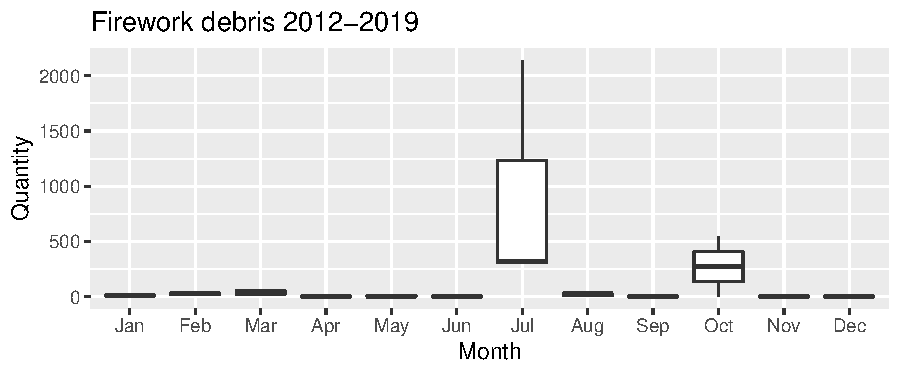
\includegraphics[width=1\linewidth]{figure/unnamed-chunk-14-1} 

\end{knitrout}
\caption {Categorisation of Rubber Glover over Time}
\label{figE1}
\end {center}
\end {figure}

However when the Rubber Glove categorisation was considered over time, it became apparent that in September 2019, the first use of "Rubber" to classify Rubber Gloves appeared as did the the last categorisation as "Plastic" at the same time. This suggests that the material classification was changed at this time, and suggested to the authors that the historically classified Rubber Gloves should be reclassified as Rubber for consistency in comparison. \hl{we should probably change all Rubber Gloves to "Rubber" to make them consistent or explain why we didn't} \\


\pagebreak
\subsection{Recategorisation}\label{recategorisation}

The \textbf{ItemName} subcategories of the Plastic type were recategorised following the CCI protocol to allow for consistency and comparability across studies as has been discussed in \hyperref[research]{Section 2}.\\

\hl{show original categories?}\\





\begin{figure}[H] 
\begin{center}

\caption {Debris by categorisation}
\label{figE}
\end {center}
\end {figure}


\begin{knitrout}\small
\definecolor{shadecolor}{rgb}{0.969, 0.969, 0.969}\color{fgcolor}\begin{kframe}
\begin{alltt}
\hlcom{# Recategorisation of all plastic items by CCI categories}

\hlcom{# all cigarette related waste: 1, 4, 6, 22}
\hlcom{# Food related waste: 3, 2,7,9,10, 17, 23, 11}
\hlcom{# Non food related waste: 8, 14, 15, 16, 18, 19, 21, 20}
\hlcom{# Plastic bags and Styrofoam packaging:12, 13}
\hlcom{# Fragments: 5, 23, 24,25}

\hlstd{recategorise} \hlkwb{<-} \hlkwa{function}\hlstd{(}\hlkwc{x}\hlstd{)\{}
  \hlstd{out} \hlkwb{=} \hlstr{""}
  \hlkwa{if}\hlstd{(x} \hlopt \hlkwd{c}\hlstd{(}\hlnum{1}\hlstd{,}\hlnum{4}\hlstd{,}\hlnum{6}\hlstd{,}\hlnum{22}\hlstd{))\{out} \hlkwb{=} \hlstr{"Cigarette related waste"}\hlstd{\}}
  \hlkwa{if}\hlstd{(x} \hlopt \hlkwd{c}\hlstd{(}\hlnum{2}\hlstd{,}\hlnum{3}\hlstd{,}\hlnum{7}\hlstd{,}\hlnum{9}\hlstd{,}\hlnum{10}\hlstd{,}\hlnum{17}\hlstd{,}\hlnum{23}\hlstd{,}\hlnum{11}\hlstd{)) out} \hlkwb{=} \hlstr{"Food related waste"}
  \hlkwa{if}\hlstd{(x} \hlopt \hlkwd{c}\hlstd{(}\hlnum{8}\hlstd{,}\hlnum{14}\hlstd{,}\hlnum{15}\hlstd{,}\hlnum{16}\hlstd{,}\hlnum{18}\hlstd{,}\hlnum{19}\hlstd{,}\hlnum{21}\hlstd{,}\hlnum{20}\hlstd{)) out} \hlkwb{=} \hlstr{"Other"}
  \hlkwa{if}\hlstd{(x} \hlopt \hlkwd{c}\hlstd{(}\hlnum{12}\hlstd{,}\hlnum{13}\hlstd{)) out} \hlkwb{=} \hlstr{"Plastic bags and Styrofoam packaging"}
  \hlkwa{if}\hlstd{(x} \hlopt \hlkwd{c}\hlstd{(}\hlnum{5}\hlstd{,}\hlnum{23}\hlstd{,}\hlnum{24}\hlstd{,}\hlnum{25}\hlstd{)) out} \hlkwb{=} \hlstr{"Fragments"}
  \hlkwa{if}\hlstd{(out} \hlopt{==} \hlstr{""}\hlstd{)} \hlkwd{stop}\hlstd{(}\hlkwd{paste}\hlstd{(}\hlstr{"Error in recategorise:"}\hlstd{, x))}
  \hlkwd{return}\hlstd{(out)}
\hlstd{\}}

\hlstd{plastic_types} \hlkwb{<-} \hlstd{data} \hlopt
  \hlkwd{filter}\hlstd{(`Material Description`} \hlopt{==} \hlstr{"PLASTIC"}\hlstd{)} \hlopt
  \hlkwd{select}\hlstd{(ItemName, ItemID)} \hlopt
  \hlkwd{distinct}\hlstd{()} \hlopt
  \hlkwd{mutate}\hlstd{(}\hlkwc{label} \hlstd{=} \hlnum{1}\hlopt{:}\hlkwd{n}\hlstd{())} \hlopt
  \hlkwd{mutate}\hlstd{(}\hlkwc{category} \hlstd{= purrr}\hlopt{::}\hlkwd{map}\hlstd{(label, recategorise))} \hlopt
  \hlkwd{mutate}\hlstd{(}\hlkwc{category} \hlstd{=} \hlkwd{as_factor}\hlstd{(}\hlkwd{as.character}\hlstd{(category)))} \hlopt
  \hlkwd{select}\hlstd{(ItemID, category)}


\hlstd{plastic} \hlkwb{<-} \hlstd{data} \hlopt
  \hlkwd{filter}\hlstd{(`Material Description`} \hlopt{==} \hlstr{"PLASTIC"}\hlstd{)} \hlopt
  \hlkwd{full_join}\hlstd{(plastic_types,} \hlkwc{by} \hlstd{=} \hlstr{"ItemID"}\hlstd{)}

\hlstd{ordered_levels} \hlkwb{<-} \hlstd{plastic} \hlopt
  \hlkwd{group_by}\hlstd{(category)} \hlopt
  \hlkwd{summarise}\hlstd{(}\hlkwc{totObs} \hlstd{=} \hlkwd{sum}\hlstd{(Quantity))} \hlopt
  \hlkwd{ungroup}\hlstd{()} \hlopt
  \hlkwd{arrange}\hlstd{(}\hlkwd{desc}\hlstd{(totObs))} \hlopt
  \hlkwd{select}\hlstd{(category)} \hlopt
  \hlstd{category}
\hlstd{plastic}\hlopt{$}\hlstd{category} \hlkwb{<-} \hlkwd{factor}\hlstd{(plastic}\hlopt{$}\hlstd{category,} \hlkwc{levels} \hlstd{= ordered_levels)}
\hlkwd{rm}\hlstd{(ordered_levels)}
\end{alltt}
\end{kframe}
\end{knitrout}

\begin{figure}[H]
\begin{center}
\begin{knitrout}\small
\definecolor{shadecolor}{rgb}{0.969, 0.969, 0.969}\color{fgcolor}\begin{kframe}
\begin{alltt}
\hlstd{plastic} \hlopt
  \hlkwd{mutate}\hlstd{(}\hlkwc{month} \hlstd{=} \hlkwd{month}\hlstd{(Time,} \hlkwc{label} \hlstd{=} \hlnum{FALSE}\hlstd{),}
         \hlkwc{year} \hlstd{=} \hlkwd{as.integer}\hlstd{(}\hlkwd{year}\hlstd{(Time)))} \hlopt
  \hlkwd{group_by}\hlstd{(month, year, category)} \hlopt
  \hlkwd{summarise}\hlstd{(}\hlkwc{`Total Quantity`} \hlstd{=} \hlkwd{sum}\hlstd{(Quantity))} \hlopt
  \hlkwd{ggplot}\hlstd{(}\hlkwd{aes}\hlstd{(}\hlkwc{x} \hlstd{= month,} \hlkwc{y} \hlstd{= `Total Quantity`,} \hlkwc{fill} \hlstd{= category))} \hlopt{+}
    \hlkwd{geom_col}\hlstd{(}\hlkwc{colour} \hlstd{=} \hlstr{"black"}\hlstd{,} \hlkwc{size} \hlstd{=} \hlnum{0.2}\hlstd{,} \hlkwc{position} \hlstd{=} \hlstr{"fill"}\hlstd{)} \hlopt{+}
    \hlkwd{facet_wrap}\hlstd{(}\hlopt{~}\hlstd{year,} \hlkwc{nrow} \hlstd{=} \hlnum{2}\hlstd{)} \hlopt{+}
    \hlkwd{scale_fill_viridis}\hlstd{(}\hlkwc{discrete} \hlstd{=} \hlnum{TRUE}\hlstd{,} \hlkwc{option} \hlstd{=} \hlstr{"plasma"}\hlstd{)} \hlopt{+}
    \hlkwd{xlab}\hlstd{(}\hlstr{"Month"}\hlstd{)} \hlopt{+}
    \hlkwd{ylab}\hlstd{(}\hlstr{"Proportion of Items"}\hlstd{)} \hlopt{+}
    \hlkwd{scale_x_continuous}\hlstd{(}\hlkwc{breaks} \hlstd{=} \hlnum{1}\hlopt{:}\hlnum{12}\hlstd{)} \hlopt{+}
    \hlkwd{theme}\hlstd{(}\hlkwc{panel.grid.major.x} \hlstd{=} \hlkwd{element_blank}\hlstd{(),}
          \hlkwc{panel.grid.minor.x} \hlstd{=} \hlkwd{element_blank}\hlstd{(),}
          \hlkwc{legend.position} \hlstd{=} \hlstr{"bottom"}\hlstd{,}
          \hlkwc{legend.text}\hlstd{=}\hlkwd{element_text}\hlstd{(}\hlkwc{size}\hlstd{=}\hlnum{5}\hlstd{))} \hlopt{+}
    \hlkwd{guides}\hlstd{(}\hlkwc{fill}\hlstd{=}\hlkwd{guide_legend}\hlstd{(}\hlkwc{title}\hlstd{=}\hlstr{"Category"}\hlstd{))}
\end{alltt}
\end{kframe}
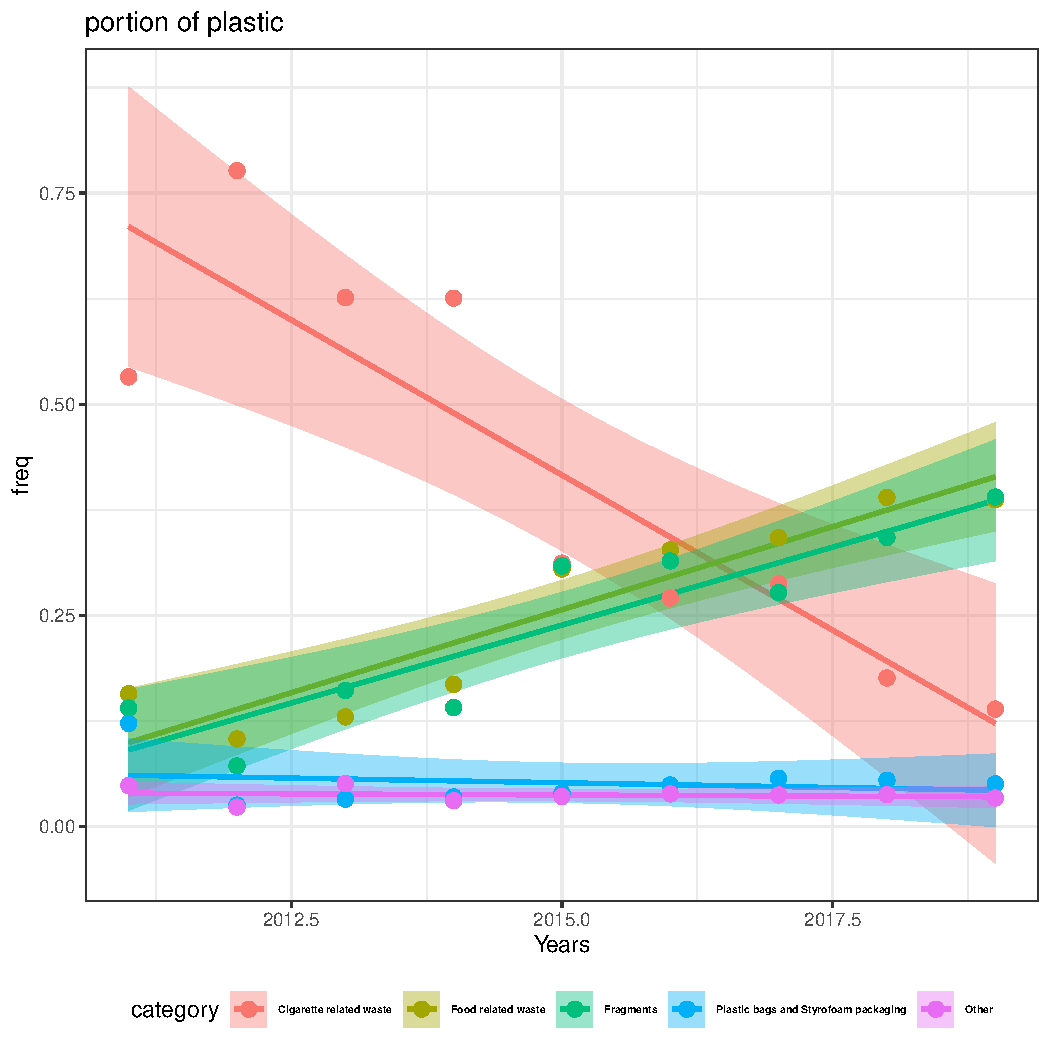
\includegraphics[width=1\linewidth]{figure/unnamed-chunk-18-1} 

\end{knitrout}
\caption {Relative frequencies of observed plastic waste by category}
\label{figB}
\end {center}
\end {figure}


















\pagebreak
\section{Experiments}



\subsection{Proportion Trends}
% The key variable in this section is TIME (Years, Months)
After cleaning and recategorisation of the data, it was analysed to determine how pollutant proportions change over time.\\

\begin{figure}[H] 
\begin{center}
\begin{knitrout}\small
\definecolor{shadecolor}{rgb}{0.969, 0.969, 0.969}\color{fgcolor}\begin{kframe}
\begin{alltt}
\hlcom{# Line chart of observations: Total v Plastic}
\hlstd{data} \hlopt
  \hlkwd{mutate}\hlstd{(}\hlkwc{Type} \hlstd{=} \hlkwd{if_else}\hlstd{(`Material Description`} \hlopt{==} \hlstr{"PLASTIC"}\hlstd{,} \hlstr{"Plastic"}\hlstd{,} \hlstr{"Other"}\hlstd{),}
         \hlkwc{months} \hlstd{=} \hlkwd{floor_date}\hlstd{(Time,} \hlstr{'month'}\hlstd{))} \hlopt
  \hlkwd{group_by}\hlstd{(months, Type)} \hlopt
  \hlkwd{summarize}\hlstd{(}\hlkwc{`Number of observations`} \hlstd{=} \hlkwd{n}\hlstd{())} \hlopt
  \hlkwd{ggplot}\hlstd{(}\hlkwd{aes}\hlstd{(}\hlkwc{x} \hlstd{= months,} \hlkwc{y} \hlstd{= `Number of observations`,} \hlkwc{colour} \hlstd{= Type))} \hlopt{+}
    \hlkwd{geom_line}\hlstd{()} \hlopt{+}
    \hlkwd{theme}\hlstd{(}\hlkwc{legend.position} \hlstd{=} \hlstr{"bottom"}\hlstd{)}
\end{alltt}
\end{kframe}
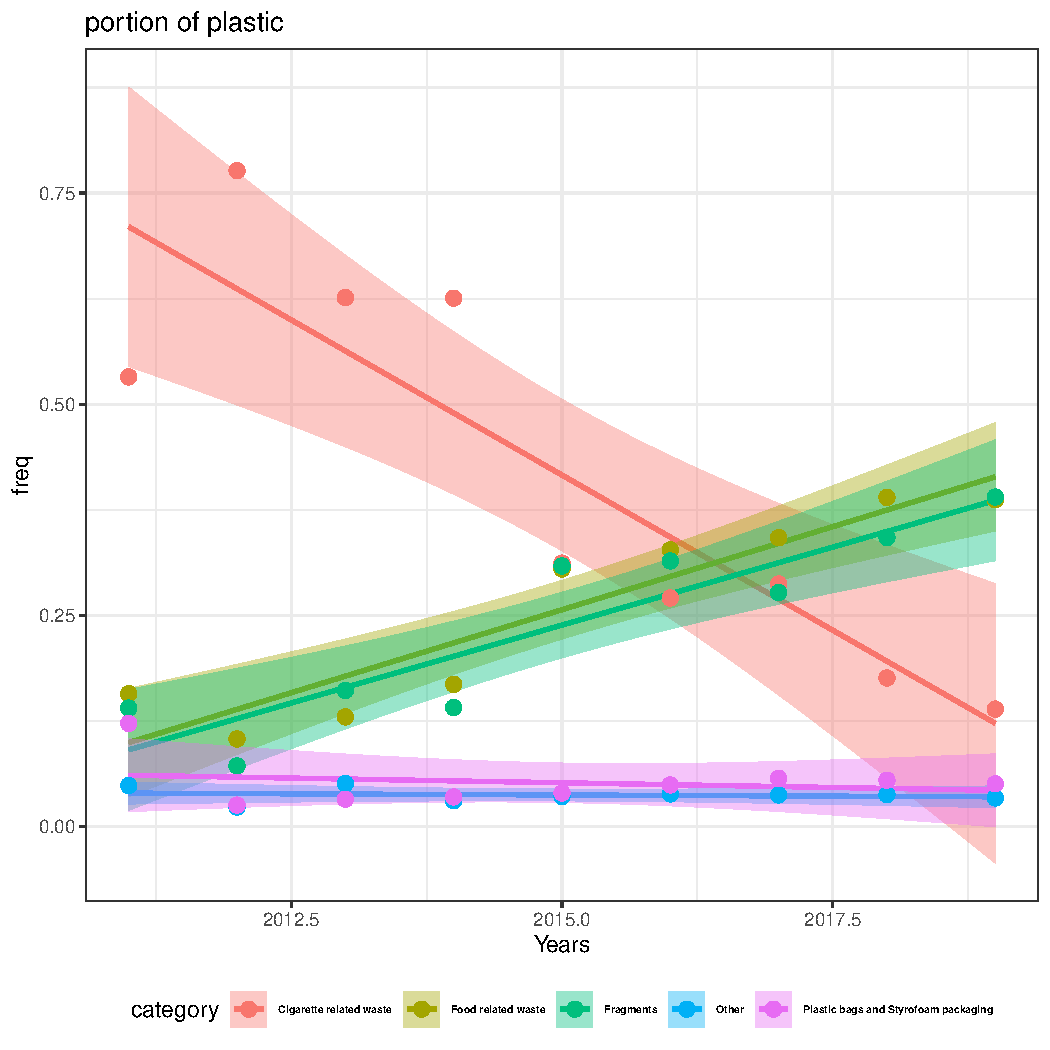
\includegraphics[width=1\linewidth]{figure/unnamed-chunk-19-1} 

\end{knitrout}
\caption {Observations of plastic debris v all debris}
\label{figF}
\end {center}
\end {figure}

In this chart we see peaks and troughs in the number of observations - this is indicative of an increase in user activity. Seeing the peak in 2013 - that's not to say pollution suddenly increased in one period and disappeared, but monitoring activity spiked in that period. \hl{do we know why?} We see more of these spikes in 2017, 2018 and 2019 but generally it is an increasing trend in monitoring activity.\\


Per the data, we see an increase in debris observed over time. Caution must be exercised in interpreting this information, as this increase may be reflective indeed of increased pollution levels, but it could also be because of increased activity in the citizen science project as it matures and gains a larger user base.

\begin{figure}[H] 
\begin{center}
\begin{knitrout}\small
\definecolor{shadecolor}{rgb}{0.969, 0.969, 0.969}\color{fgcolor}\begin{kframe}
\begin{alltt}
\hlcom{#Linechart quantity of debris per year}
\hlstd{data} \hlopt
  \hlkwd{mutate}\hlstd{(}\hlkwc{year} \hlstd{=} \hlkwd{year}\hlstd{(Time))} \hlopt
  \hlkwd{group_by}\hlstd{(year)} \hlopt
  \hlkwd{summarise}\hlstd{(}\hlkwc{quan} \hlstd{=} \hlkwd{sum}\hlstd{(Quantity))} \hlopt
  \hlkwd{ggplot}\hlstd{(}\hlkwd{aes}\hlstd{(}\hlkwc{x} \hlstd{= year,} \hlkwc{y} \hlstd{= quan))} \hlopt{+}
    \hlkwd{geom_col}\hlstd{()} \hlopt{+}
    \hlkwd{scale_x_continuous}\hlstd{(}\hlkwc{breaks} \hlstd{=} \hlnum{2012}\hlopt{:}\hlnum{2019}\hlstd{)} \hlopt{+}
    \hlkwd{xlab}\hlstd{(}\hlstr{"Year"}\hlstd{)} \hlopt{+}
    \hlkwd{ylab}\hlstd{(}\hlstr{"Quantity"}\hlstd{)} \hlopt{+}
    \hlkwd{scale_y_continuous}\hlstd{(}\hlkwc{labels} \hlstd{= scales}\hlopt{::}\hlkwd{label_number_si}\hlstd{(}\hlkwc{accuracy} \hlstd{=} \hlnum{1}\hlstd{))} \hlopt{+}
    \hlkwd{theme}\hlstd{(}\hlkwc{panel.grid.major.x} \hlstd{=} \hlkwd{element_blank}\hlstd{(),}
          \hlkwc{panel.grid.minor.x} \hlstd{=} \hlkwd{element_blank}\hlstd{())}
\end{alltt}
\end{kframe}
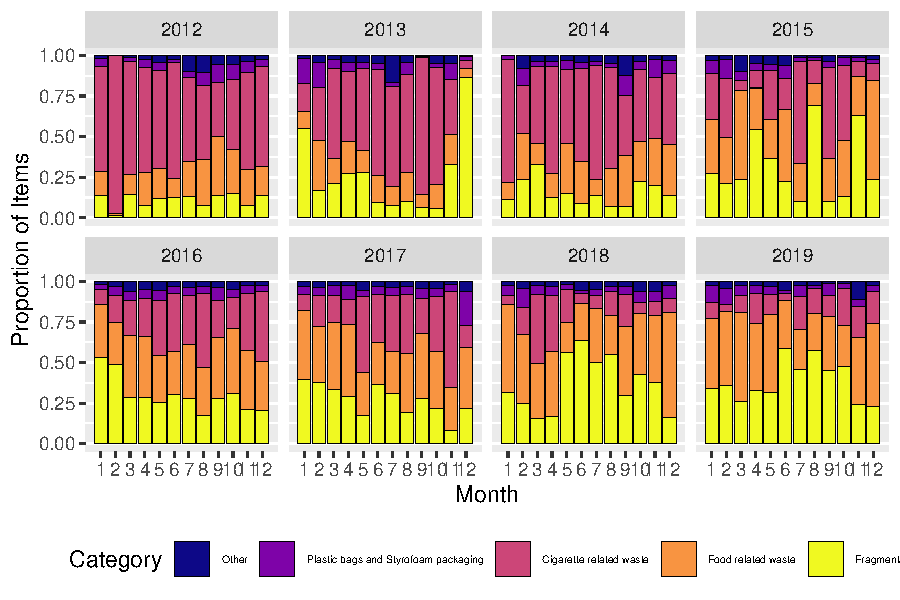
\includegraphics[width=1\linewidth]{figure/unnamed-chunk-20-1} 

\end{knitrout}
\caption {Quantity of debris per year}
\label{figD}
\end {center}
\end {figure}

\begin{figure}[H] 
\begin{center}
\begin{knitrout}\small
\definecolor{shadecolor}{rgb}{0.969, 0.969, 0.969}\color{fgcolor}\begin{kframe}
\begin{alltt}
\hlcom{# Column plot of average daily observations by year}
\hlstd{data} \hlopt
  \hlkwd{mutate}\hlstd{(}\hlkwc{Date} \hlstd{=} \hlkwd{date}\hlstd{(Time))} \hlopt
  \hlkwd{full_join}\hlstd{(}\hlkwd{tibble}\hlstd{(}\hlkwc{Date} \hlstd{=} \hlkwd{full_seq}\hlstd{(}\hlkwd{c}\hlstd{(}\hlkwd{min}\hlstd{(}\hlkwd{date}\hlstd{(data}\hlopt{$}\hlstd{Time)),} \hlkwd{max}\hlstd{(}\hlkwd{date}\hlstd{(data}\hlopt{$}\hlstd{Time))),} \hlkwc{period} \hlstd{=} \hlnum{1}\hlstd{)),} \hlkwc{by} \hlstd{=} \hlstr{"Date"}\hlstd{)} \hlopt \hlcom{# Check for any missing days}
  \hlkwd{group_by}\hlstd{(Date)} \hlopt
  \hlkwd{summarise}\hlstd{(}\hlkwc{Observations} \hlstd{=} \hlkwd{length}\hlstd{(LogID))} \hlopt
  \hlkwd{ungroup}\hlstd{()} \hlopt
  \hlkwd{mutate}\hlstd{(}\hlkwc{Year} \hlstd{= lubridate}\hlopt{::}\hlkwd{year}\hlstd{(Date))} \hlopt
  \hlkwd{group_by}\hlstd{(Year)} \hlopt
  \hlkwd{summarise}\hlstd{(}\hlkwc{Average_Daily_Observations} \hlstd{=} \hlkwd{mean}\hlstd{(Observations))} \hlopt
  \hlkwd{ungroup}\hlstd{()} \hlopt
  \hlkwd{ggplot}\hlstd{(}\hlkwd{aes}\hlstd{(}\hlkwc{x} \hlstd{= Year,} \hlkwc{y} \hlstd{= Average_Daily_Observations))} \hlopt{+}
    \hlkwd{geom_col}\hlstd{()} \hlopt{+}
    \hlkwd{xlab}\hlstd{(}\hlstr{"Year"}\hlstd{)} \hlopt{+}
    \hlkwd{ylab}\hlstd{(}\hlstr{"Average Daily Observations"}\hlstd{)} \hlopt{+}
    \hlkwd{scale_x_continuous}\hlstd{(}\hlkwc{breaks} \hlstd{=} \hlnum{2012}\hlopt{:}\hlnum{2019}\hlstd{)} \hlopt{+}
    \hlkwd{theme_bw}\hlstd{()} \hlopt{+}
    \hlkwd{theme}\hlstd{(}\hlkwc{text} \hlstd{=} \hlkwd{element_text}\hlstd{(}\hlkwc{size}\hlstd{=}\hlnum{8}\hlstd{),}
          \hlkwc{panel.grid.major} \hlstd{=} \hlkwd{element_blank}\hlstd{(),}
          \hlkwc{panel.grid.minor} \hlstd{=} \hlkwd{element_blank}\hlstd{())}
\end{alltt}
\end{kframe}
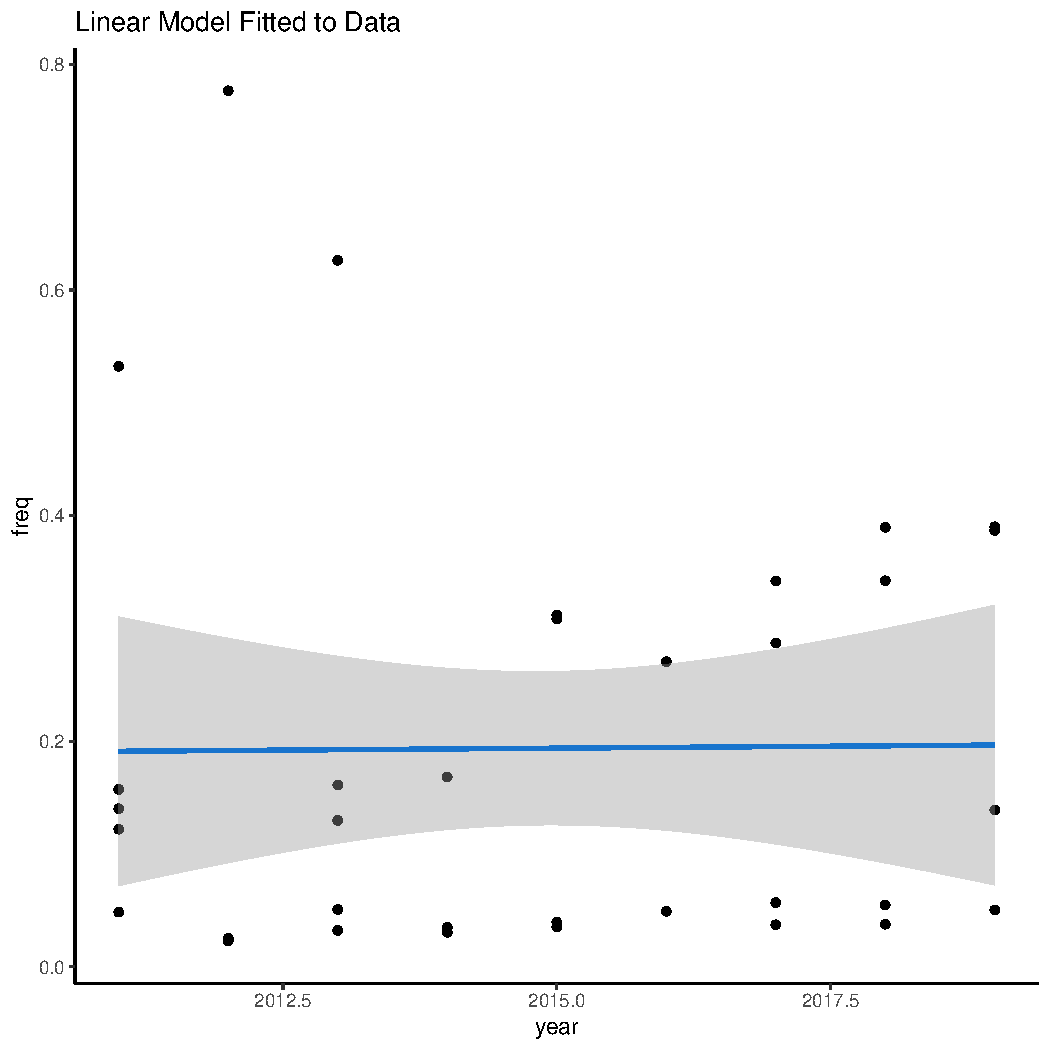
\includegraphics[width=1\linewidth]{figure/unnamed-chunk-21-1} 

\end{knitrout}
\caption {Average Daily Observations by Year}
\label{figD1}
\end {center}
\end {figure}

As we see in the chart above, an increase in the number of average observations per day lends support to the theory that the increase in observations is factored by increase in citizen science monitoring activity. That's not to say pollution has not also increased in this period, but it would be inaccurate to not account for the increase in monitoring activity.\\

\hl{can we put the above two charts together, side by side or top/bottom?}\\


\begin{figure}[H] 
\begin{center}
\begin{knitrout}\small
\definecolor{shadecolor}{rgb}{0.969, 0.969, 0.969}\color{fgcolor}\begin{kframe}
\begin{alltt}
\hlcom{# Column chart showing % distribution of material types}
\hlstd{data} \hlopt
  \hlkwd{mutate}\hlstd{(}\hlkwc{Year} \hlstd{= lubridate}\hlopt{::}\hlkwd{year}\hlstd{(Time))} \hlopt
  \hlkwd{group_by}\hlstd{(Year, `Material Description`)} \hlopt
  \hlkwd{summarise}\hlstd{(}\hlkwc{Counts} \hlstd{=} \hlkwd{n}\hlstd{())} \hlopt
  \hlkwd{ungroup}\hlstd{()} \hlopt
  \hlkwd{ggplot}\hlstd{(}\hlkwd{aes}\hlstd{(}\hlkwc{x} \hlstd{= Year,} \hlkwc{y} \hlstd{= Counts,} \hlkwc{fill} \hlstd{= `Material Description`))} \hlopt{+}
    \hlkwd{geom_col}\hlstd{(}\hlkwc{colour} \hlstd{=} \hlstr{"black"}\hlstd{,} \hlkwc{size} \hlstd{=} \hlnum{0.2}\hlstd{,} \hlkwc{position} \hlstd{=} \hlstr{"fill"}\hlstd{)} \hlopt{+}
    \hlkwd{scale_fill_hue}\hlstd{(}\hlkwc{l}\hlstd{=}\hlnum{50}\hlstd{,} \hlkwc{c}\hlstd{=}\hlnum{150}\hlstd{)} \hlopt{+}
    \hlkwd{scale_x_continuous}\hlstd{(}\hlkwc{breaks} \hlstd{=} \hlnum{2012}\hlopt{:}\hlnum{2019}\hlstd{)} \hlopt{+}
    \hlkwd{scale_y_continuous}\hlstd{(}\hlkwc{labels}\hlstd{=scales}\hlopt{::}\hlstd{percent,} \hlkwc{name}\hlstd{=}\hlstr{""}\hlstd{)} \hlopt{+}
    \hlkwd{theme_bw}\hlstd{()} \hlopt{+}
    \hlkwd{theme}\hlstd{(}\hlkwc{text} \hlstd{=} \hlkwd{element_text}\hlstd{(}\hlkwc{size}\hlstd{=}\hlnum{8}\hlstd{),}
          \hlkwc{panel.grid.major} \hlstd{=} \hlkwd{element_blank}\hlstd{(),}
          \hlkwc{panel.grid.minor} \hlstd{=} \hlkwd{element_blank}\hlstd{(),}
          \hlkwc{legend.position} \hlstd{=} \hlstr{"bottom"}\hlstd{)}
\end{alltt}
\end{kframe}
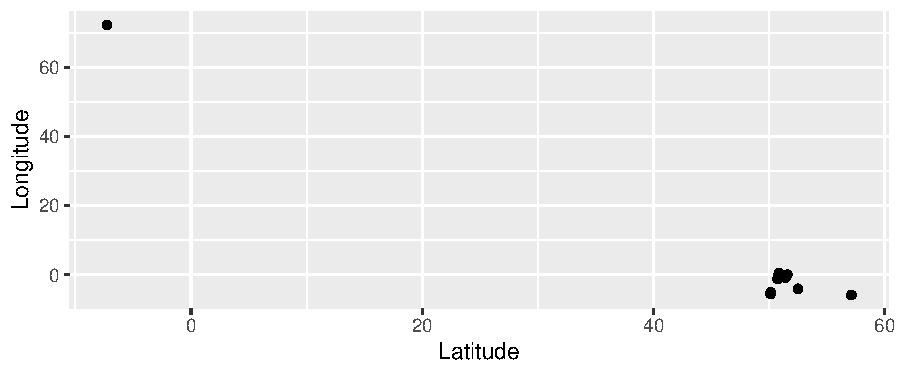
\includegraphics[width=1\linewidth]{figure/unnamed-chunk-22-1} 

\end{knitrout}
\caption {Proportion of Debris by Material Types}
\label{fig1}
\end {center}
\end {figure}

Analysis of the poportions of pollutant materials identifies that plastic is the dominant marine pollutant material, and its majority proportion of total debris is relatively consistent year on year. This could be due to an increase in new plastic pollution entering marine environments from source, not helped by the fact it is durable and does not decompose quickly, or that the other pollutant materials are decreasing. This analysis therefore is in agreement with the studies discussed in \hyperref[research]{Section 2} that plastic is indeed the biggest problem in marine pollution accounting for approximately 70\% of all marine pollution. 




\begin{figure}[H] 
\begin{center}
\begin{knitrout}\small
\definecolor{shadecolor}{rgb}{0.969, 0.969, 0.969}\color{fgcolor}\begin{kframe}
\begin{alltt}
\hlcom{# Line of just Plastic}
\hlstd{data} \hlopt
  \hlkwd{mutate}\hlstd{(}\hlkwc{Year} \hlstd{= lubridate}\hlopt{::}\hlkwd{year}\hlstd{(Time))} \hlopt
  \hlkwd{group_by}\hlstd{(Year, `Material Description`)} \hlopt
  \hlkwd{summarise}\hlstd{(}\hlkwc{total} \hlstd{=} \hlkwd{n}\hlstd{())} \hlopt
  \hlkwd{mutate}\hlstd{(}\hlkwc{prop} \hlstd{= total} \hlopt{/} \hlkwd{sum}\hlstd{(total),}\hlkwc{lab}\hlstd{=scales}\hlopt{::}\hlkwd{percent}\hlstd{(prop))} \hlopt
  \hlkwd{filter}\hlstd{(`Material Description`}\hlopt{==}\hlstr{"PLASTIC"}\hlstd{)} \hlopt
  \hlkwd{ggplot}\hlstd{(}\hlkwd{aes}\hlstd{(}\hlkwc{x} \hlstd{= Year,} \hlkwc{y} \hlstd{= prop,} \hlkwc{label} \hlstd{= lab))}\hlopt{+}
  \hlkwd{geom_text}\hlstd{(}\hlkwc{nudge_y} \hlstd{=} \hlnum{0.05}\hlstd{,} \hlkwc{color} \hlstd{=} \hlstr{"black"}\hlstd{)} \hlopt{+}
  \hlkwd{geom_line}\hlstd{(}\hlkwd{aes}\hlstd{(}\hlkwc{x} \hlstd{= Year,} \hlkwc{y} \hlstd{= prop))}\hlopt{+}
  \hlkwd{geom_point}\hlstd{(}\hlkwd{aes}\hlstd{(}\hlkwc{x} \hlstd{= Year,} \hlkwc{y} \hlstd{= prop))} \hlopt{+}
  \hlkwd{scale_y_continuous}\hlstd{(}\hlkwc{labels}\hlstd{=scales}\hlopt{::}\hlstd{percent,} \hlkwc{name}\hlstd{=}\hlstr{""}\hlstd{,} \hlkwc{limits} \hlstd{=} \hlkwd{c}\hlstd{(}\hlnum{0}\hlstd{,} \hlnum{1}\hlstd{))} \hlopt{+}
  \hlkwd{theme_bw}\hlstd{()} \hlopt{+}
  \hlkwd{theme}\hlstd{(}\hlkwc{panel.grid.major} \hlstd{=} \hlkwd{element_blank}\hlstd{(),}
        \hlkwc{panel.grid.minor} \hlstd{=} \hlkwd{element_blank}\hlstd{(),}
        \hlkwc{legend.position} \hlstd{=} \hlstr{"bottom"}\hlstd{)}
\end{alltt}
\end{kframe}
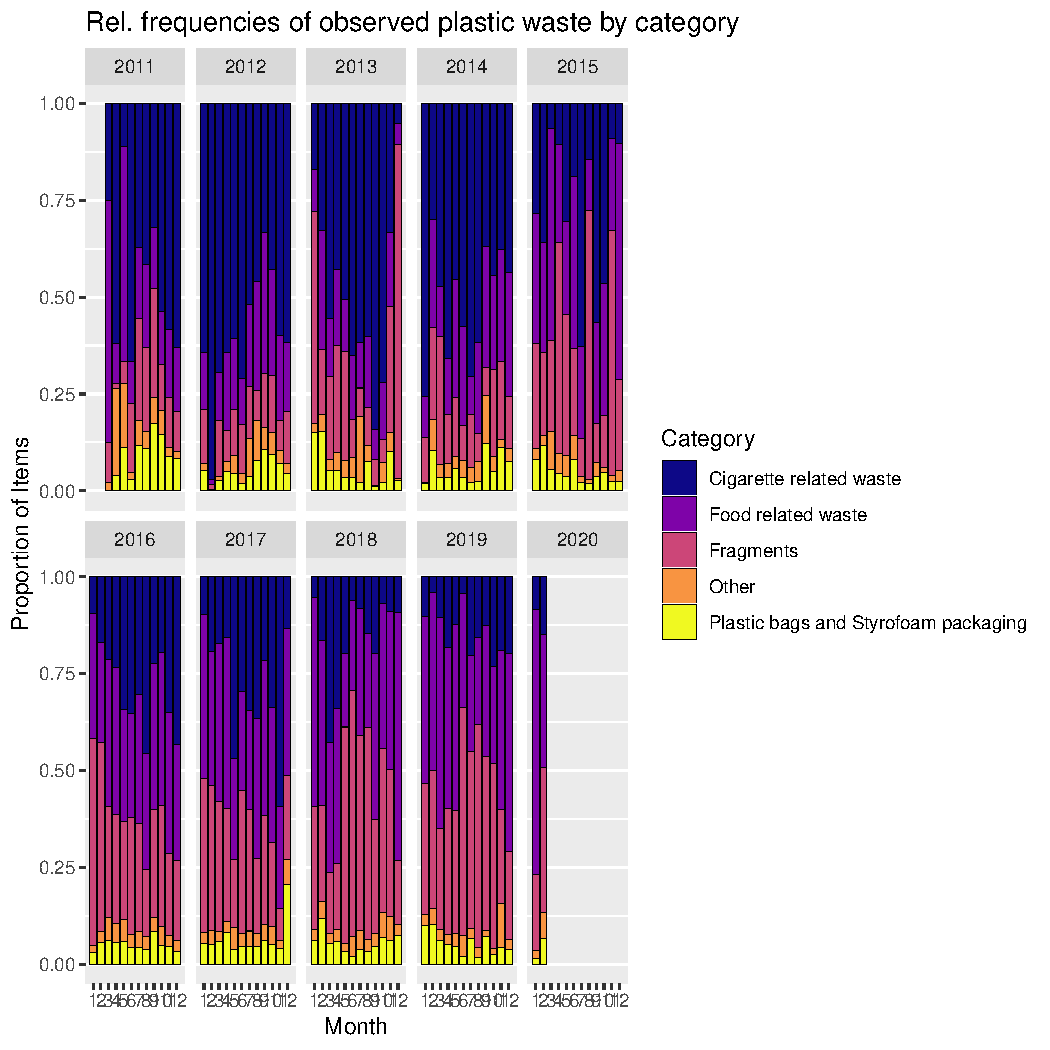
\includegraphics[width=1\linewidth]{figure/unnamed-chunk-23-1} 

\end{knitrout}
\caption {Trend of Plastic as a proportion of Total Debris}
\label{figF}
\end {center}
\end {figure}

When considering the charts above, it can be determined that even as total debris observations increase, so do plastic observations which means plastics remain a consistently common feature of the observed derbis over time.\\

\begin{figure}[H] 
\begin{center}
\begin{knitrout}\small
\definecolor{shadecolor}{rgb}{0.969, 0.969, 0.969}\color{fgcolor}\begin{kframe}
\begin{alltt}
\hlcom{# Facet of categories}
\hlstd{plastic} \hlopt
  \hlkwd{filter}\hlstd{(`Material Description`} \hlopt{==} \hlstr{"PLASTIC"}\hlstd{)} \hlopt
  \hlkwd{mutate}\hlstd{(} \hlkwc{year} \hlstd{=} \hlkwd{as.integer}\hlstd{(}\hlkwd{year}\hlstd{(Time)))} \hlopt
  \hlkwd{group_by}\hlstd{(year, category)} \hlopt
  \hlkwd{summarise}\hlstd{(}\hlkwc{total} \hlstd{=} \hlkwd{n}\hlstd{())} \hlopt
  \hlkwd{mutate}\hlstd{(}\hlkwc{prop} \hlstd{= total} \hlopt{/} \hlkwd{sum}\hlstd{(total),}\hlkwc{lab}\hlstd{=scales}\hlopt{::}\hlkwd{percent}\hlstd{(prop))} \hlopt
  \hlkwd{ggplot}\hlstd{(}\hlkwd{aes}\hlstd{(}\hlkwc{x} \hlstd{= year,} \hlkwc{y} \hlstd{= prop))} \hlopt{+}
    \hlkwd{geom_line}\hlstd{()} \hlopt{+}
    \hlkwd{facet_wrap}\hlstd{(}\hlopt{~}\hlstd{category,} \hlkwc{nrow} \hlstd{=} \hlnum{2}\hlstd{)} \hlopt{+}
    \hlkwd{theme}\hlstd{(}\hlkwc{axis.text.y} \hlstd{=} \hlkwd{element_blank}\hlstd{(),}
          \hlkwc{axis.title.x} \hlstd{=} \hlkwd{element_blank}\hlstd{(),}
          \hlkwc{axis.title.y} \hlstd{=} \hlkwd{element_blank}\hlstd{())}
\end{alltt}
\end{kframe}
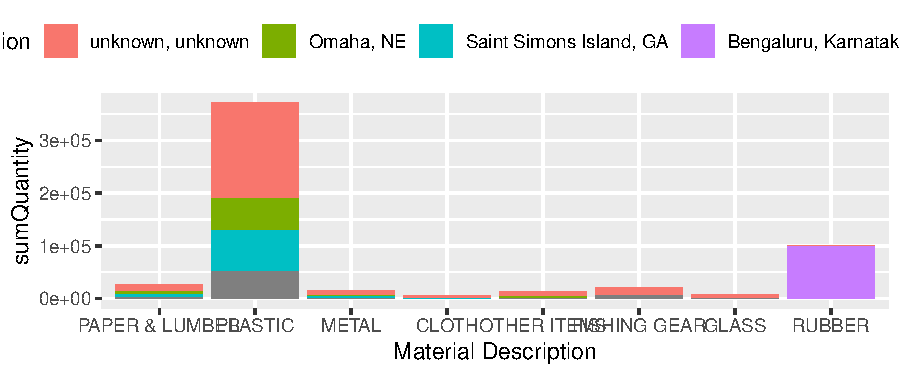
\includegraphics[width=1\linewidth]{figure/unnamed-chunk-24-1} 

\end{knitrout}
\caption {Proportion of Plastic Items Over Time}
\label{figF3}
\end {center}
\end {figure}

\begin{figure}[H] 
\begin{center}
\begin{knitrout}\small
\definecolor{shadecolor}{rgb}{0.969, 0.969, 0.969}\color{fgcolor}\begin{kframe}
\begin{alltt}
\hlcom{# Line chart of CCI categorised plastics}
\hlstd{plastic} \hlopt
  \hlkwd{mutate}\hlstd{(}\hlkwc{Year} \hlstd{= lubridate}\hlopt{::}\hlkwd{year}\hlstd{(Time))} \hlopt
  \hlkwd{group_by}\hlstd{(Year, category)} \hlopt
  \hlkwd{summarise}\hlstd{(}\hlkwc{total} \hlstd{=} \hlkwd{n}\hlstd{())} \hlopt
  \hlkwd{mutate}\hlstd{(}\hlkwc{prop} \hlstd{= total} \hlopt{/} \hlkwd{sum}\hlstd{(total),}\hlkwc{lab}\hlstd{=scales}\hlopt{::}\hlkwd{percent}\hlstd{(prop))} \hlopt
  \hlkwd{ggplot}\hlstd{(}\hlkwd{aes}\hlstd{(}\hlkwc{x} \hlstd{= Year,} \hlkwc{y} \hlstd{= prop,} \hlkwc{color} \hlstd{= category,} \hlkwc{label} \hlstd{= lab))}\hlopt{+}
  \hlcom{#geom_text(color = "black") + }
  \hlkwd{geom_line}\hlstd{(}\hlkwd{aes}\hlstd{(}\hlkwc{x} \hlstd{= Year,} \hlkwc{y} \hlstd{= prop,} \hlkwc{color} \hlstd{= category))}\hlopt{+}
  \hlkwd{geom_point}\hlstd{(}\hlkwd{aes}\hlstd{(}\hlkwc{x} \hlstd{= Year,} \hlkwc{y} \hlstd{= prop,} \hlkwc{color} \hlstd{= category))} \hlopt{+}
  \hlkwd{scale_y_continuous}\hlstd{(}\hlkwc{labels}\hlstd{=scales}\hlopt{::}\hlstd{percent,} \hlkwc{name}\hlstd{=}\hlstr{""}\hlstd{,} \hlkwc{limits} \hlstd{=} \hlkwd{c}\hlstd{(}\hlnum{0}\hlstd{,} \hlnum{1}\hlstd{))} \hlopt{+}
  \hlkwd{theme_bw}\hlstd{()} \hlopt{+}
  \hlkwd{theme}\hlstd{(}\hlkwc{panel.grid.major} \hlstd{=} \hlkwd{element_blank}\hlstd{(),}
        \hlkwc{panel.grid.minor} \hlstd{=} \hlkwd{element_blank}\hlstd{(),}
        \hlkwc{legend.position} \hlstd{=} \hlstr{"bottom"}\hlstd{)}
\end{alltt}
\end{kframe}
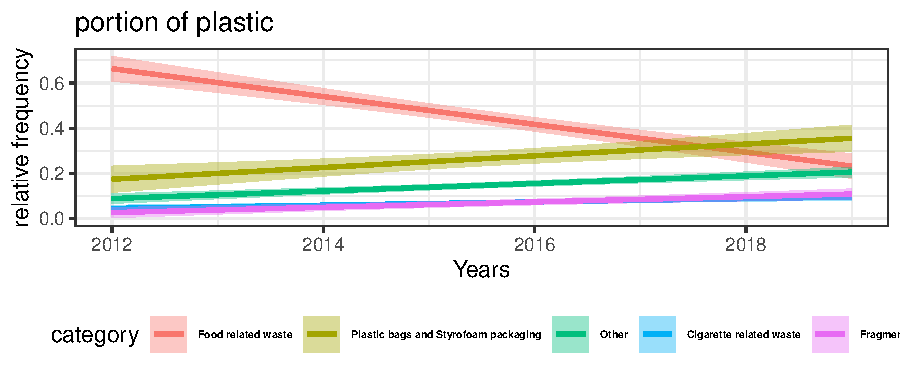
\includegraphics[width=1\linewidth]{figure/unnamed-chunk-25-1} 

\end{knitrout}
\caption {Trend of Plastic Proportions by CCI Categories}
\label{figF}
\end {center}
\end {figure}

\begin{figure}[H] 
\begin{center}
\begin{knitrout}\small
\definecolor{shadecolor}{rgb}{0.969, 0.969, 0.969}\color{fgcolor}\begin{kframe}
\begin{alltt}
\hlstd{data} \hlopt
  \hlkwd{filter}\hlstd{(`Material Description`} \hlopt{==} \hlstr{"PLASTIC"}\hlstd{)} \hlopt
  \hlkwd{mutate}\hlstd{(}\hlkwc{year} \hlstd{=} \hlkwd{as.integer}\hlstd{(}\hlkwd{year}\hlstd{(Time)))} \hlopt
  \hlkwd{group_by}\hlstd{(year, ItemName)} \hlopt
  \hlkwd{summarise}\hlstd{(}\hlkwc{total} \hlstd{=} \hlkwd{n}\hlstd{())} \hlopt
  \hlkwd{mutate}\hlstd{(}\hlkwc{prop} \hlstd{= total} \hlopt{/} \hlkwd{sum}\hlstd{(total),}\hlkwc{lab}\hlstd{=scales}\hlopt{::}\hlkwd{percent}\hlstd{(prop))} \hlopt
  \hlkwd{ggplot}\hlstd{(}\hlkwd{aes}\hlstd{(}\hlkwc{x} \hlstd{= year,} \hlkwc{y} \hlstd{= prop))} \hlopt{+}
    \hlkwd{geom_line}\hlstd{()} \hlopt{+}
    \hlkwd{scale_y_continuous}\hlstd{(}\hlkwc{labels}\hlstd{=scales}\hlopt{::}\hlstd{percent,} \hlkwc{name}\hlstd{=}\hlstr{"% of Total Plastic"}\hlstd{)} \hlopt{+}
    \hlkwd{facet_wrap}\hlstd{(}\hlopt{~}\hlstd{ItemName,} \hlkwc{nrow} \hlstd{=} \hlnum{5}\hlstd{)} \hlopt{+}
    \hlkwd{theme}\hlstd{(}\hlkwc{text} \hlstd{=} \hlkwd{element_text}\hlstd{(}\hlkwc{size}\hlstd{=}\hlnum{6}\hlstd{),}
          \hlkwc{axis.text.x}\hlstd{=}\hlkwd{element_text}\hlstd{(}\hlkwc{angle}\hlstd{=}\hlnum{45}\hlstd{,} \hlkwc{hjust}\hlstd{=}\hlnum{1}\hlstd{),}
          \hlkwc{axis.ticks.y} \hlstd{=} \hlkwd{element_blank}\hlstd{(),}
          \hlkwc{axis.title.x} \hlstd{=} \hlkwd{element_blank}\hlstd{(),}
          \hlkwc{axis.title.y} \hlstd{=} \hlkwd{element_blank}\hlstd{())}
\end{alltt}
\end{kframe}
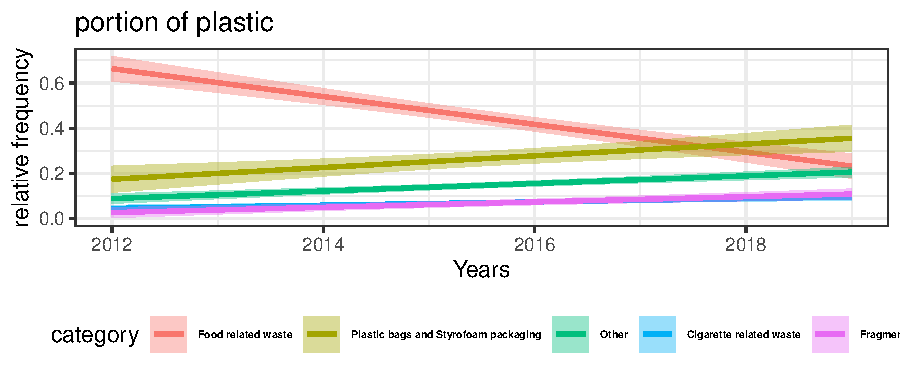
\includegraphics[width=1\linewidth]{figure/unnamed-chunk-26-1} 

\end{knitrout}
\caption {Proportion of Plastic Items Over Time}
\label{figF4}
\end {center}
\end {figure}


As these charts consider the proportion of the subcategory item of total plastics, it is important to note that the increase in Plastic or Foam fragments and Food Wrappers might be attributed actually to a decrease in other subcategories such as Cigarettes. Essentially, not that these items are becoming increasingly common, but that the share between them is levelling. Considering the discussions above, it should be recalled that all debris and plastic are being increasingly observed, so a decrease in a subcategory item is welcomed yet more must be done. To explain the decrease, it is possible that better waste management practices for cigarettes have been put into place, for example the introduction of penalties for literring cigarette butts or installing better cigarette butt collection points in high activity areas, resulting the decrease of observations witnessed here. It could however also be influenced by changes in social patterns such as persons smoking less or moving to reusable portable vaping devices which result is the lower consumption of single-use cigarettes and the resulting debris. Eitherway, being able to view key subcategories like this allows researchers to identify where to focus their efforts to ultimately achieve the aim of reducing pollution. 

\pagebreak
\subsection {Distribution of observed debris:}
% The key variable in this section is PROPORTIONS %

\begin{figure}[H] 
\begin{center}
\begin{knitrout}\small
\definecolor{shadecolor}{rgb}{0.969, 0.969, 0.969}\color{fgcolor}\begin{kframe}
\begin{alltt}
\hlcom{# Column chart of Debris Quantity by Material Type}
\hlstd{data} \hlopt \hlkwd{select}\hlstd{(Description,`Material Description`)} \hlopt
  \hlkwd{group_by}\hlstd{(`Material Description`)} \hlopt
  \hlkwd{summarise}\hlstd{(}\hlkwc{Observed} \hlstd{=} \hlkwd{n}\hlstd{())} \hlopt
  \hlkwd{ggplot}\hlstd{(}\hlkwd{aes}\hlstd{(}\hlkwc{x} \hlstd{=} \hlkwd{reorder}\hlstd{(`Material Description`,} \hlopt{-}\hlstd{Observed),} \hlkwc{y} \hlstd{= Observed))} \hlopt{+}
    \hlkwd{geom_col}\hlstd{()} \hlopt{+}
    \hlkwd{ylab}\hlstd{(}\hlstr{"Total observed"}\hlstd{)} \hlopt{+}
    \hlkwd{xlab}\hlstd{(}\hlstr{"Material"}\hlstd{)} \hlopt{+}
    \hlkwd{theme}\hlstd{(}\hlkwc{text} \hlstd{=} \hlkwd{element_text}\hlstd{(}\hlkwc{size}\hlstd{=}\hlnum{8}\hlstd{),}
        \hlkwc{axis.text.x}\hlstd{=}\hlkwd{element_text}\hlstd{(}\hlkwc{angle}\hlstd{=}\hlnum{45}\hlstd{,} \hlkwc{hjust}\hlstd{=}\hlnum{1}\hlstd{),}
        \hlkwc{plot.title} \hlstd{=} \hlkwd{element_text}\hlstd{(}\hlkwc{size}\hlstd{=}\hlnum{10}\hlstd{))}
\end{alltt}
\end{kframe}
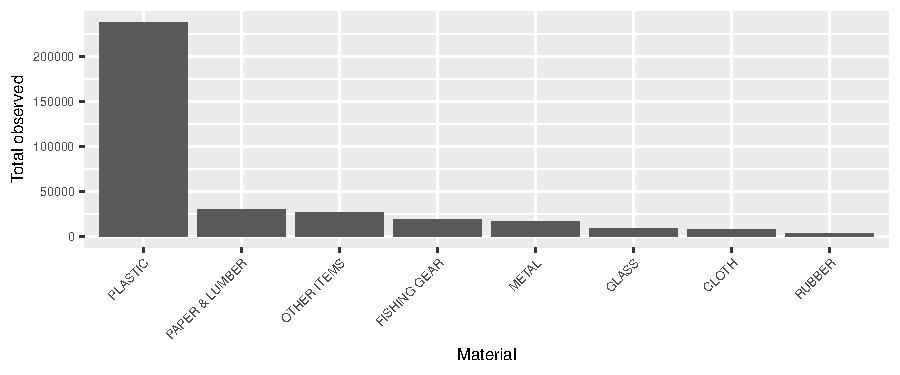
\includegraphics[width=1\linewidth]{figure/unnamed-chunk-27-1} 
\begin{kframe}\begin{alltt}
    \hlcom{#coord_flip()}
\end{alltt}
\end{kframe}
\end{knitrout}
\caption {Material Quantities}
\label{figC}
\end {center}
\end {figure}

The most populated material class is Plastic. Note that this does not necessarily mean that plastic is the largest quantity of debris, just that the individual number of items categorised is largest.


\begin{figure}[H] 
\begin{center}
\begin{knitrout}\small
\definecolor{shadecolor}{rgb}{0.969, 0.969, 0.969}\color{fgcolor}\begin{kframe}
\begin{alltt}
\hlcom{# Treemap of debris categories}
\hlstd{data} \hlopt
  \hlkwd{select}\hlstd{(`Material Description`, ItemName, Quantity)} \hlopt
  \hlkwd{group_by}\hlstd{(`Material Description`, ItemName)} \hlopt
  \hlkwd{summarise}\hlstd{(}\hlkwc{Quantity} \hlstd{=} \hlkwd{sum}\hlstd{(Quantity))} \hlopt
  \hlkwd{treemap}\hlstd{(}\hlkwc{index} \hlstd{=} \hlkwd{c}\hlstd{(}\hlstr{"Material Description"}\hlstd{,} \hlstr{"ItemName"}\hlstd{),}
          \hlkwc{vSize} \hlstd{=} \hlstr{"Quantity"}\hlstd{,} \hlkwc{draw} \hlstd{=} \hlnum{TRUE}\hlstd{)} \hlkwb{->} \hlstd{tm}
\end{alltt}
\end{kframe}
\end{knitrout}
\caption {Debris categorisation}
\label{figI}
\end {center}
\end {figure}





\begin{figure}[H] 
\begin{center}
\begin{knitrout}\small
\definecolor{shadecolor}{rgb}{0.969, 0.969, 0.969}\color{fgcolor}\begin{kframe}
\begin{alltt}
\hlcom{#bar of debris categories}
\hlstd{data} \hlopt
  \hlkwd{select}\hlstd{(`Material Description`, ItemName)} \hlopt
  \hlkwd{group_by}\hlstd{(`Material Description`, ItemName)} \hlopt
  \hlkwd{summarise}\hlstd{(}\hlkwc{Observed} \hlstd{=} \hlkwd{n}\hlstd{())} \hlopt
  \hlkwd{arrange}\hlstd{(}\hlkwd{desc}\hlstd{(Observed))} \hlopt
  \hlkwd{head}\hlstd{(}\hlnum{15}\hlstd{)} \hlopt
  \hlkwd{ggplot}\hlstd{(}\hlkwd{aes}\hlstd{(}\hlkwc{x}\hlstd{=}\hlkwd{reorder}\hlstd{(`ItemName`,} \hlopt{-}\hlstd{Observed),} \hlkwc{y}\hlstd{=Observed,} \hlkwc{fill}\hlstd{=`Material Description`))} \hlopt{+}
  \hlkwd{geom_bar}\hlstd{(}\hlkwc{stat}\hlstd{=}\hlstr{"identity"}\hlstd{)} \hlopt{+}
  \hlkwd{xlab}\hlstd{(}\hlstr{"Debris"}\hlstd{)} \hlopt{+}
  \hlkwd{ylab}\hlstd{(}\hlstr{""}\hlstd{)} \hlopt{+}
  \hlcom{#coord_flip() +}
  \hlkwd{theme}\hlstd{(}\hlkwc{text} \hlstd{=} \hlkwd{element_text}\hlstd{(}\hlkwc{size}\hlstd{=}\hlnum{8}\hlstd{),}
        \hlkwc{axis.text.x}\hlstd{=}\hlkwd{element_text}\hlstd{(}\hlkwc{angle}\hlstd{=}\hlnum{45}\hlstd{,} \hlkwc{hjust}\hlstd{=}\hlnum{1}\hlstd{),}
        \hlkwc{legend.text}\hlstd{=}\hlkwd{element_text}\hlstd{(}\hlkwc{size}\hlstd{=}\hlnum{5}\hlstd{),}
        \hlkwc{legend.position} \hlstd{=} \hlstr{"bottom"}\hlstd{)}
\end{alltt}
\end{kframe}
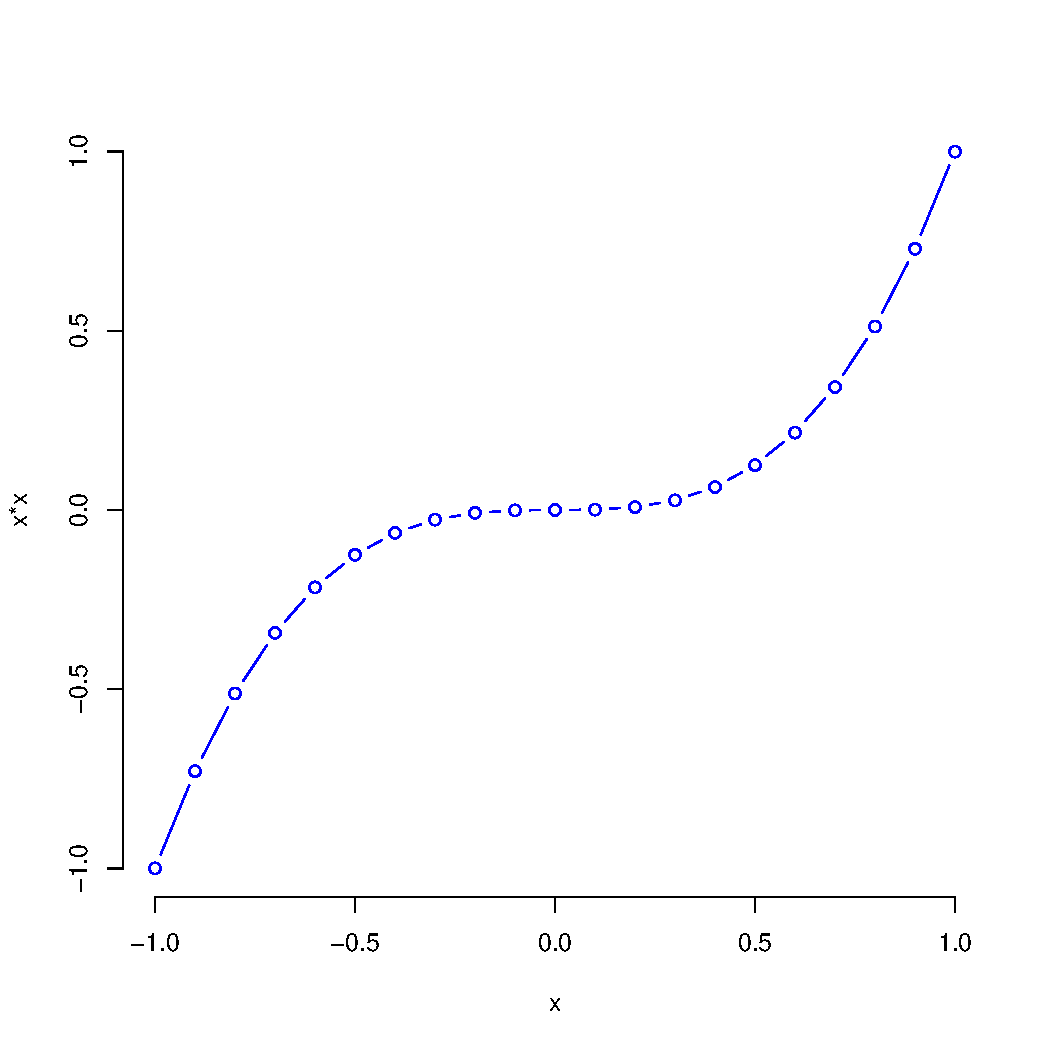
\includegraphics[width=1\linewidth]{figure/unnamed-chunk-29-1} 

\end{knitrout}
\caption {Top 15 Debris Items Observed between 2012 and 2019}
\label{figI2}
\end {center}
\end {figure}


Does this align with the other studies discussed in \hyperref[research]{Section 2} where the main items identified were plastic bags, and in one study specifically from India which found cigarettes was actually their smallest pollutant at 5.5\% \cite{KUMAR2016}. 




\pagebreak
\subsection{Location-Driven Pollution}

Here we see that the dataset is global, yet with a heavy influence in America. We also see that while most observed locations are on the coastline, some make reference to oceanic bodies, and some are inland, which would account for pollution also observed in rivers and freshwater marine environments like lakes and natural reservoirs.

\begin{knitrout}\small
\definecolor{shadecolor}{rgb}{0.969, 0.969, 0.969}\color{fgcolor}\begin{kframe}
\begin{alltt}
\hlcom{# Map of all observed locations}
\hlstd{world} \hlkwb{<-} \hlkwd{map_data}\hlstd{(}\hlstr{"world"}\hlstd{)}
\hlstd{data} \hlopt
  \hlkwd{select}\hlstd{(Latitude, Longitude)} \hlopt
  \hlkwd{ggplot}\hlstd{()} \hlopt{+}
    \hlkwd{geom_polygon}\hlstd{(}\hlkwc{data} \hlstd{=} \hlkwd{map_data}\hlstd{(}\hlstr{"world"}\hlstd{),} \hlkwd{aes}\hlstd{(}\hlkwc{x} \hlstd{= long,} \hlkwc{y} \hlstd{= lat,} \hlkwc{group} \hlstd{= group),} \hlkwc{fill} \hlstd{=} \hlstr{"grey"}\hlstd{,} \hlkwc{alpha} \hlstd{=} \hlnum{0.5}\hlstd{)} \hlopt{+}
    \hlkwd{geom_hex}\hlstd{(}\hlkwd{aes}\hlstd{(}\hlkwc{x} \hlstd{= Longitude,} \hlkwc{y} \hlstd{= Latitude),} \hlkwc{bins} \hlstd{=} \hlnum{50}\hlstd{)} \hlopt{+}
    \hlkwd{scale_fill_viridis}\hlstd{(}\hlkwc{trans} \hlstd{=} \hlstr{"log"}\hlstd{,} \hlkwc{breaks} \hlstd{=} \hlkwd{c}\hlstd{(}\hlnum{5}\hlstd{,} \hlnum{50}\hlstd{,} \hlnum{500}\hlstd{,} \hlnum{5000}\hlstd{,} \hlnum{50000}\hlstd{))} \hlopt{+}
    \hlkwd{theme_void}\hlstd{()} \hlopt{+}
    \hlkwd{guides}\hlstd{(}\hlkwc{fill}\hlstd{=}\hlkwd{guide_legend}\hlstd{(}\hlkwc{title}\hlstd{=}\hlstr{"Observations"}\hlstd{))} \hlopt{+}
    \hlkwd{theme}\hlstd{(}\hlkwc{plot.title} \hlstd{=} \hlkwd{element_text}\hlstd{(}\hlkwc{size}\hlstd{=}\hlnum{10}\hlstd{),}
      \hlkwc{text} \hlstd{=} \hlkwd{element_text}\hlstd{(}\hlkwc{size}\hlstd{=}\hlnum{8}\hlstd{),}
      \hlkwc{panel.grid.major} \hlstd{=} \hlkwd{element_blank}\hlstd{(),}
      \hlkwc{panel.grid.minor} \hlstd{=} \hlkwd{element_blank}\hlstd{(),}
      \hlkwc{legend.position} \hlstd{=} \hlstr{"bottom"}\hlstd{)}
\end{alltt}
\end{kframe}
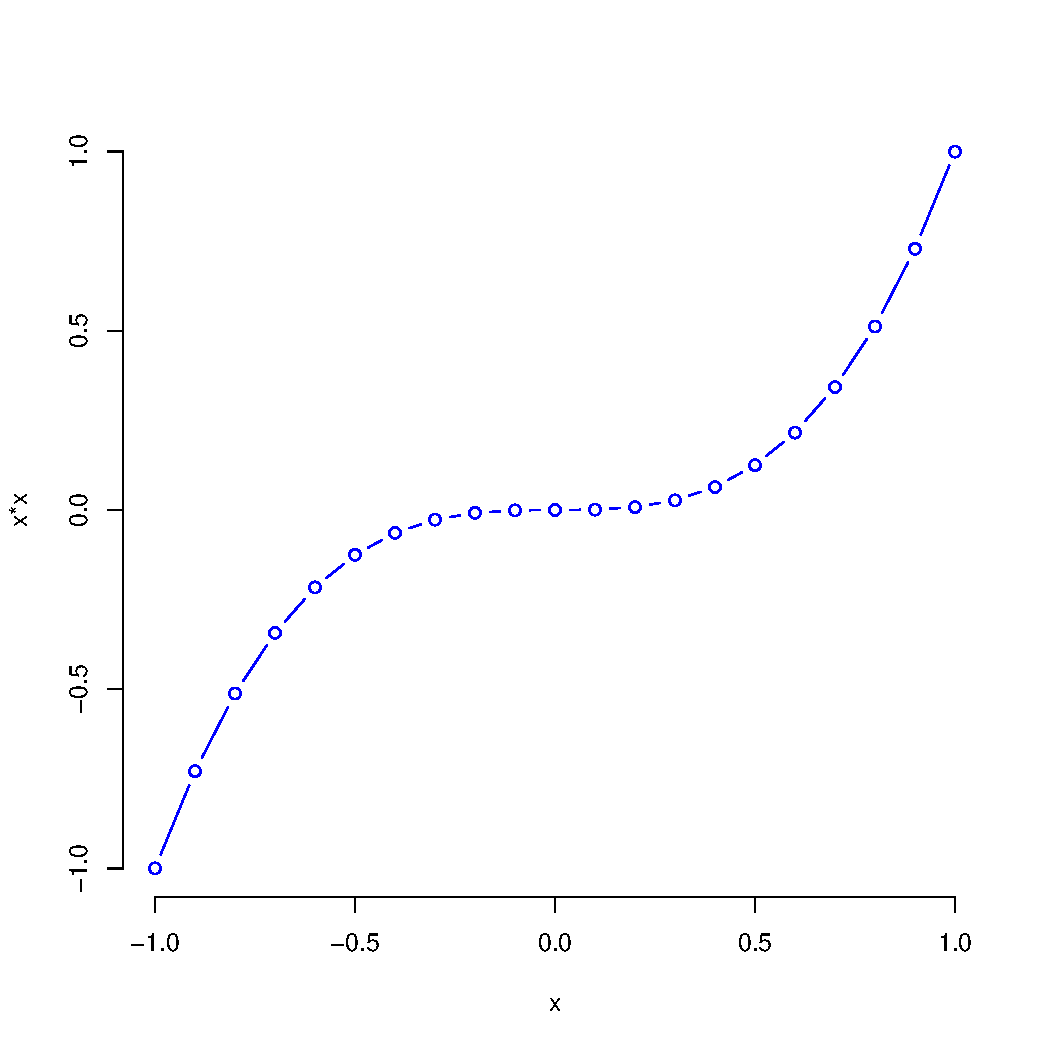
\includegraphics[width=1\linewidth]{figure/unnamed-chunk-30-1} 

\end{knitrout}


\begin{figure}[H] 
\begin{center}
\begin{knitrout}\small
\definecolor{shadecolor}{rgb}{0.969, 0.969, 0.969}\color{fgcolor}\begin{kframe}
\begin{alltt}
\hlcom{#columnchart of debris locations}
\hlstd{topLocations} \hlkwb{<-} \hlstd{data} \hlopt
  \hlkwd{group_by}\hlstd{(Location)} \hlopt
  \hlkwd{summarise}\hlstd{(}\hlkwc{Observed} \hlstd{=} \hlkwd{n}\hlstd{())} \hlopt
  \hlkwd{arrange}\hlstd{(}\hlkwd{desc}\hlstd{(Observed))} \hlopt
  \hlkwd{top_n}\hlstd{(}\hlnum{15}\hlstd{,Observed)}

\hlstd{data} \hlopt
  \hlcom{#filter(Location %in% topLocations$Location) %>% }
  \hlkwd{group_by}\hlstd{(Location, `Material Description`)} \hlopt
  \hlkwd{summarise}\hlstd{(}\hlkwc{Observed} \hlstd{=} \hlkwd{n}\hlstd{())} \hlopt
  \hlkwd{arrange}\hlstd{(}\hlkwd{desc}\hlstd{(Observed))} \hlopt
  \hlkwd{head}\hlstd{(}\hlnum{100}\hlstd{)} \hlopt
  \hlkwd{ggplot}\hlstd{(}\hlkwd{aes}\hlstd{(}\hlkwc{x} \hlstd{= Location,} \hlkwc{y} \hlstd{= Observed,} \hlkwc{fill} \hlstd{= `Material Description`))} \hlopt{+}
    \hlkwd{geom_col}\hlstd{(}\hlkwc{colour} \hlstd{=} \hlstr{"black"}\hlstd{,} \hlkwc{size} \hlstd{=} \hlnum{0.2}\hlstd{,} \hlkwc{position} \hlstd{=} \hlstr{"fill"}\hlstd{)} \hlopt{+}
    \hlkwd{scale_y_continuous}\hlstd{(}\hlkwc{labels}\hlstd{=scales}\hlopt{::}\hlstd{percent,} \hlkwc{name}\hlstd{=}\hlstr{""}\hlstd{)} \hlopt{+}
    \hlkwd{theme_bw}\hlstd{()} \hlopt{+}
    \hlkwd{theme}\hlstd{(}\hlkwc{text} \hlstd{=} \hlkwd{element_text}\hlstd{(}\hlkwc{size}\hlstd{=}\hlnum{8}\hlstd{),}
          \hlkwc{axis.text.x}\hlstd{=}\hlkwd{element_text}\hlstd{(}\hlkwc{angle}\hlstd{=}\hlnum{45}\hlstd{,} \hlkwc{hjust}\hlstd{=}\hlnum{1}\hlstd{),}
          \hlkwc{panel.grid.major} \hlstd{=} \hlkwd{element_blank}\hlstd{(),}
          \hlkwc{panel.grid.minor} \hlstd{=} \hlkwd{element_blank}\hlstd{(),}
          \hlkwc{legend.position} \hlstd{=} \hlstr{"bottom"}\hlstd{)}
\end{alltt}
\end{kframe}
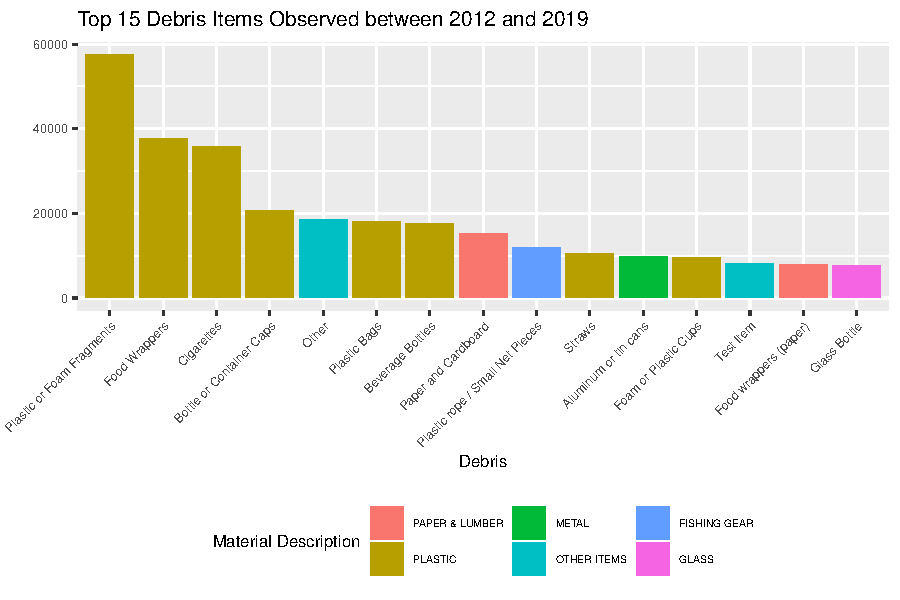
\includegraphics[width=1\linewidth]{figure/unnamed-chunk-31-1} 

\end{knitrout}
\caption {Debris by location}
\label{figG}
\end {center}
\end {figure}


\pagebreak
\subsection{Event-Driven Pollution}

An interesting pattern which emerged when conducting exploratory analysis on the data, were peaks in the observations of debris classified as Fireworks consistently in July.\\

\begin{figure}[H] 
\begin{center}
\begin{knitrout}\small
\definecolor{shadecolor}{rgb}{0.969, 0.969, 0.969}\color{fgcolor}\begin{kframe}
\begin{alltt}
\hlcom{# Boxplot of fireworks distribution by month (across all years)}
\hlstd{data} \hlopt
  \hlkwd{filter}\hlstd{(`Material Description`} \hlopt{==} \hlstr{"PLASTIC"}\hlstd{,}
         \hlstd{ItemName} \hlopt \hlkwd{c}\hlstd{(}\hlstr{"Fireworks"}\hlstd{))} \hlopt
  \hlkwd{mutate}\hlstd{(}\hlkwc{month} \hlstd{=} \hlkwd{month}\hlstd{(Time,} \hlkwc{label} \hlstd{=} \hlnum{TRUE}\hlstd{),}
         \hlkwc{year} \hlstd{=} \hlkwd{as.integer}\hlstd{(}\hlkwd{year}\hlstd{(Time)))} \hlopt
  \hlkwd{group_by}\hlstd{(month, year)} \hlopt
  \hlkwd{summarise}\hlstd{(}\hlkwc{Observed} \hlstd{=} \hlkwd{n}\hlstd{())} \hlopt
  \hlkwd{ggplot}\hlstd{()} \hlopt{+}
    \hlkwd{geom_boxplot}\hlstd{(}\hlkwd{aes}\hlstd{(}\hlkwc{x} \hlstd{= month,} \hlkwc{y} \hlstd{= Observed))} \hlopt{+}
    \hlkwd{xlab}\hlstd{(}\hlstr{"Month"}\hlstd{)} \hlopt{+}
    \hlkwd{ylab}\hlstd{(}\hlstr{"Observed"}\hlstd{)} \hlopt{+}
    \hlkwd{theme_bw}\hlstd{()} \hlopt{+}
    \hlkwd{theme}\hlstd{(}\hlkwc{text} \hlstd{=} \hlkwd{element_text}\hlstd{(}\hlkwc{size}\hlstd{=}\hlnum{8}\hlstd{),}
      \hlkwc{panel.grid.major} \hlstd{=} \hlkwd{element_blank}\hlstd{(),}
      \hlkwc{panel.grid.minor} \hlstd{=} \hlkwd{element_blank}\hlstd{(),}
      \hlkwc{legend.position} \hlstd{=} \hlstr{"bottom"}\hlstd{)}
\end{alltt}
\end{kframe}
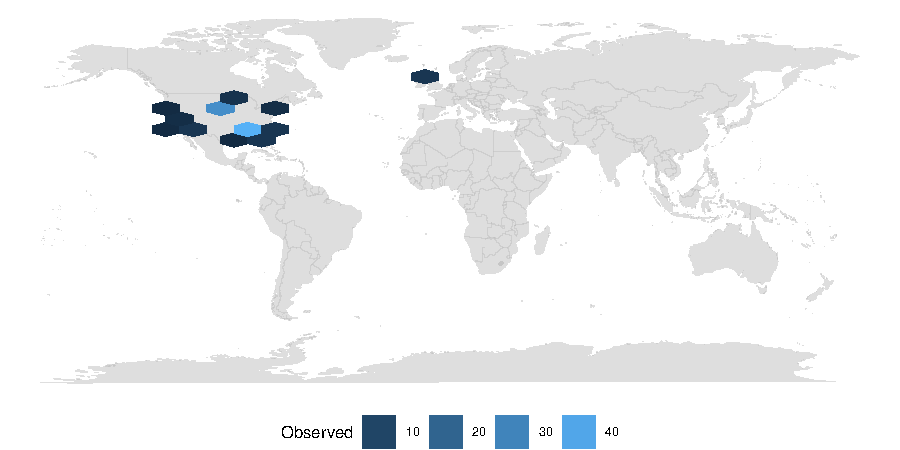
\includegraphics[width=1\linewidth]{figure/unnamed-chunk-32-1} 

\end{knitrout}
\caption {Firework debris 2012-2019}
\label{figA1}
\end {center}
\end {figure}

Given that it is known the dataset is heavily American influence, a theory emerged that the spikes of observed debris were possibly related to American 4th of July celebrations. Looking at the locations of the firework observations certainly seemed to support that. Interestingly, no spikes are observed in January which might suggest New years' celebrations, or in November for Bonfire Night celebrations on the 5th of November in the UK.\\

This gives rise to the idea that plastic pollution while sometimes blamed to be the effect of manufacturing processes, can also be largely driven by the disposable behaviours which humans encourage in these one off-events, where the items are not intended for repeated use. Used once and discarded, sadly finding its way into marine environments.


\begin{figure}[H] 
\begin{center}    
\begin{knitrout}\small
\definecolor{shadecolor}{rgb}{0.969, 0.969, 0.969}\color{fgcolor}\begin{kframe}
\begin{alltt}
\hlcom{# Map of locations having observed firework debris}
\hlstd{data} \hlopt
  \hlkwd{filter}\hlstd{(ItemName} \hlopt{==} \hlstr{"Fireworks"}\hlstd{)} \hlopt
  \hlkwd{select}\hlstd{(Latitude, Longitude)} \hlopt
  \hlkwd{ggplot}\hlstd{()} \hlopt{+}
    \hlkwd{geom_polygon}\hlstd{(}\hlkwc{data} \hlstd{=} \hlkwd{map_data}\hlstd{(}\hlstr{"world"}\hlstd{),} \hlkwd{aes}\hlstd{(}\hlkwc{x} \hlstd{= long,} \hlkwc{y} \hlstd{= lat,} \hlkwc{group} \hlstd{= group),} \hlkwc{fill} \hlstd{=} \hlstr{"grey"}\hlstd{,} \hlkwc{alpha} \hlstd{=} \hlnum{0.5}\hlstd{)} \hlopt{+}
    \hlkwd{geom_hex}\hlstd{(}\hlkwd{aes}\hlstd{(}\hlkwc{x} \hlstd{= Longitude,} \hlkwc{y} \hlstd{= Latitude))} \hlopt{+}
    \hlkwd{theme_void}\hlstd{()} \hlopt{+}
    \hlkwd{guides}\hlstd{(}\hlkwc{fill}\hlstd{=}\hlkwd{guide_legend}\hlstd{(}\hlkwc{title}\hlstd{=}\hlstr{"Observed"}\hlstd{))} \hlopt{+}
    \hlkwd{theme}\hlstd{(}\hlkwc{plot.title} \hlstd{=} \hlkwd{element_text}\hlstd{(}\hlkwc{size}\hlstd{=}\hlnum{10}\hlstd{),}
      \hlkwc{text} \hlstd{=} \hlkwd{element_text}\hlstd{(}\hlkwc{size}\hlstd{=}\hlnum{8}\hlstd{),}
      \hlkwc{panel.grid.major} \hlstd{=} \hlkwd{element_blank}\hlstd{(),}
      \hlkwc{panel.grid.minor} \hlstd{=} \hlkwd{element_blank}\hlstd{(),}
      \hlkwc{legend.position} \hlstd{=} \hlstr{"bottom"}\hlstd{)}
\end{alltt}
\end{kframe}
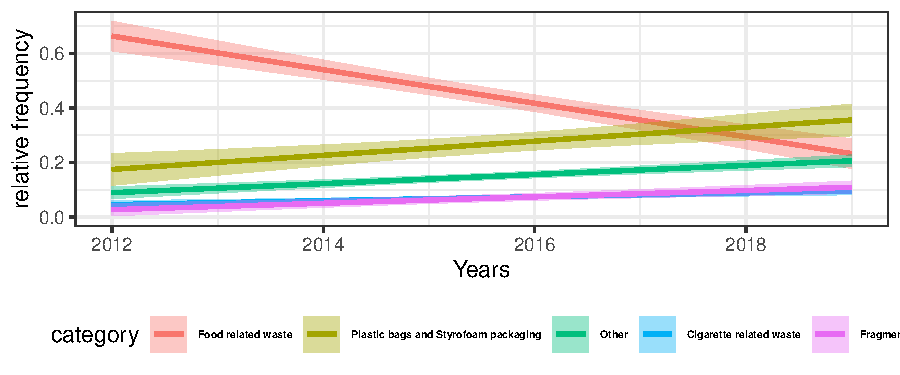
\includegraphics[width=1\linewidth]{figure/unnamed-chunk-33-1} 

\end{knitrout}

\caption {Boxplot of fireworks distribution by month, across all years}
\label{figA2}
\end {center}
\end {figure}



\pagebreak
\section{Predictive Modelling}
Given the variability of plastic pollution trends given event-driven and location-driven pollution as explored earlier in this report, the authors of this report built a model to give more accurate predictions of expected pollution levels which can be used as a base model to assess the effectiveness of pollution reducing initiatives introduced.

\subsection{Description of Model}

\begin{knitrout}\small
\definecolor{shadecolor}{rgb}{0.969, 0.969, 0.969}\color{fgcolor}\begin{kframe}
\begin{alltt}
\hlstd{plasticN} \hlkwb{<-} \hlstd{plastic} \hlopt
  \hlkwd{mutate}\hlstd{(}\hlkwc{month} \hlstd{=} \hlkwd{month}\hlstd{(Time,} \hlkwc{label} \hlstd{=} \hlnum{FALSE}\hlstd{),} \hlkwc{year} \hlstd{=} \hlkwd{as.integer}\hlstd{(}\hlkwd{year}\hlstd{(Time)))} \hlopt  \hlkwd{group_by}\hlstd{(year, category, month)} \hlopt
  \hlkwd{summarise}\hlstd{(}\hlkwc{`Total Quantity`} \hlstd{=} \hlkwd{sum}\hlstd{(Quantity))}

\hlcom{####}

\hlstd{df12N} \hlkwb{<-} \hlstd{plasticN}  \hlopt
  \hlkwd{filter}\hlstd{(year} \hlopt{==} \hlnum{2012}\hlstd{)} \hlopt
  \hlkwd{group_by}\hlstd{(year, month)} \hlopt
  \hlkwd{mutate}\hlstd{(}\hlkwc{freq} \hlstd{= `Total Quantity`} \hlopt{/} \hlkwd{sum}\hlstd{(`Total Quantity`))}

\hlstd{df13N} \hlkwb{<-} \hlstd{plasticN}  \hlopt
  \hlkwd{filter}\hlstd{(year} \hlopt{==} \hlnum{2013}\hlstd{)} \hlopt
  \hlkwd{group_by}\hlstd{(year, month)} \hlopt
  \hlkwd{mutate}\hlstd{(}\hlkwc{freq} \hlstd{= `Total Quantity`} \hlopt{/} \hlkwd{sum}\hlstd{(`Total Quantity`))}

\hlstd{df14N} \hlkwb{<-} \hlstd{plasticN}  \hlopt
  \hlkwd{filter}\hlstd{(year} \hlopt{==} \hlnum{2014}\hlstd{)} \hlopt
  \hlkwd{group_by}\hlstd{(year, month)} \hlopt
  \hlkwd{mutate}\hlstd{(}\hlkwc{freq} \hlstd{= `Total Quantity`} \hlopt{/} \hlkwd{sum}\hlstd{(`Total Quantity`))}

\hlstd{df15N} \hlkwb{<-} \hlstd{plasticN}  \hlopt
  \hlkwd{filter}\hlstd{(year} \hlopt{==} \hlnum{2015}\hlstd{)} \hlopt
  \hlkwd{group_by}\hlstd{(year, month)} \hlopt
  \hlkwd{mutate}\hlstd{(}\hlkwc{freq} \hlstd{= `Total Quantity`} \hlopt{/} \hlkwd{sum}\hlstd{(`Total Quantity`))}

\hlstd{df16N} \hlkwb{<-} \hlstd{plasticN}  \hlopt
  \hlkwd{filter}\hlstd{(year} \hlopt{==} \hlnum{2016}\hlstd{)} \hlopt
  \hlkwd{group_by}\hlstd{(year, month)} \hlopt
  \hlkwd{mutate}\hlstd{(}\hlkwc{freq} \hlstd{= `Total Quantity`} \hlopt{/} \hlkwd{sum}\hlstd{(`Total Quantity`))}

\hlstd{df17N} \hlkwb{<-} \hlstd{plasticN}  \hlopt
  \hlkwd{filter}\hlstd{(year} \hlopt{==} \hlnum{2017}\hlstd{)} \hlopt
  \hlkwd{group_by}\hlstd{(year, month)} \hlopt
  \hlkwd{mutate}\hlstd{(}\hlkwc{freq} \hlstd{= `Total Quantity`} \hlopt{/} \hlkwd{sum}\hlstd{(`Total Quantity`))}

\hlstd{df18N} \hlkwb{<-} \hlstd{plasticN}  \hlopt
  \hlkwd{filter}\hlstd{(year} \hlopt{==} \hlnum{2018}\hlstd{)} \hlopt
  \hlkwd{group_by}\hlstd{(year, month)} \hlopt
  \hlkwd{mutate}\hlstd{(}\hlkwc{freq} \hlstd{= `Total Quantity`} \hlopt{/} \hlkwd{sum}\hlstd{(`Total Quantity`))}

\hlstd{df19N} \hlkwb{<-} \hlstd{plasticN}  \hlopt
  \hlkwd{filter}\hlstd{(year} \hlopt{==} \hlnum{2019}\hlstd{)} \hlopt
  \hlkwd{group_by}\hlstd{(year, month)} \hlopt
  \hlkwd{mutate}\hlstd{(}\hlkwc{freq} \hlstd{= `Total Quantity`} \hlopt{/} \hlkwd{sum}\hlstd{(`Total Quantity`))}

\hlstd{dfTotN} \hlkwb{<-} \hlkwd{rbind}\hlstd{(df12N, df13N, df14N, df15N, df16N, df17N, df18N, df19N)}
\end{alltt}
\end{kframe}
\end{knitrout}

\begin{figure}[H] 
\begin{center}
\begin{knitrout}\small
\definecolor{shadecolor}{rgb}{0.969, 0.969, 0.969}\color{fgcolor}\begin{kframe}
\begin{alltt}
\hlcom{# plot for observing the data}
\hlstd{(time_plotfr2N} \hlkwb{<-} \hlkwd{ggplot}\hlstd{(dfTotN,} \hlkwd{aes}\hlstd{(}\hlkwc{x} \hlstd{= year,} \hlkwc{y} \hlstd{= freq,} \hlkwc{color}\hlstd{=category,} \hlkwc{fill} \hlstd{= category))} \hlopt{+}
  \hlkwd{geom_smooth}\hlstd{(}\hlkwc{method}\hlstd{=}\hlstr{"lm"}\hlstd{,} \hlkwc{level}\hlstd{=}\hlnum{0.95}\hlstd{)} \hlopt{+}
  \hlkwd{theme_bw}\hlstd{()} \hlopt{+}
  \hlkwd{xlab}\hlstd{(}\hlstr{"Years"}\hlstd{)} \hlopt{+}
  \hlkwd{ylab}\hlstd{(}\hlstr{"relative frequency"}\hlstd{)} \hlopt{+}
  \hlkwd{expand_limits}\hlstd{(}\hlkwc{y}\hlstd{=}\hlnum{0}\hlstd{)} \hlopt{+}
  \hlkwd{scale_y_continuous}\hlstd{()} \hlopt{+}
  \hlkwd{scale_x_continuous}\hlstd{()}\hlopt{+}
  \hlkwd{theme}\hlstd{(}\hlkwc{legend.position}\hlstd{=}\hlstr{"bottom"}\hlstd{)}\hlopt{+}
  \hlkwd{theme}\hlstd{(}\hlkwc{legend.text} \hlstd{=} \hlkwd{element_text}\hlstd{(}\hlkwc{size}\hlstd{=}\hlnum{5}\hlstd{,} \hlkwc{face}\hlstd{=}\hlstr{"bold"}\hlstd{)))}
\end{alltt}
\end{kframe}
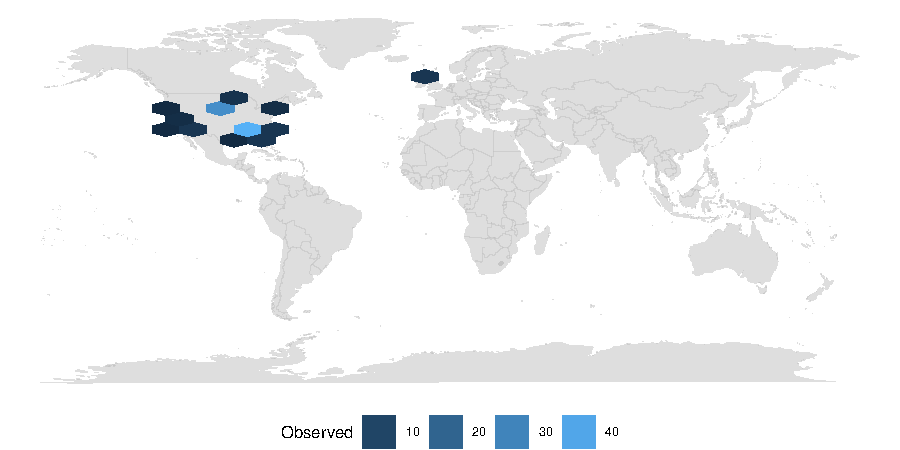
\includegraphics[width=1\linewidth]{figure/unnamed-chunk-35-1} 

\end{knitrout}
\caption {Portion of plastic}
\label{figG1}
\end {center}
\end {figure}


In this graphical representation of the relative frequency of the 5 different categories of plastic debris over the years, the insight to derive is that "Cigarette related waste, "Food related waste" and "Fragments" seem to experience some change, whereas "Other" and "Plastic bags and styrofoam packaging" seem to remain steady. A model is then created and tested on untrained data to see the early indications still stand.

\begin{knitrout}\small
\definecolor{shadecolor}{rgb}{0.969, 0.969, 0.969}\color{fgcolor}\begin{kframe}
\begin{alltt}
\hlcom{# create train and test set}
\hlstd{n} \hlkwb{<-} \hlkwd{nrow}\hlstd{(dfTotN)}  \hlcom{# Number of observations}
\hlstd{ntrain} \hlkwb{<-} \hlkwd{round}\hlstd{(n}\hlopt{*}\hlnum{0.75}\hlstd{)}  \hlcom{# 75% for training set}
\hlkwd{set.seed}\hlstd{(}\hlnum{314}\hlstd{)}    \hlcom{# Set seed for reproducible results}
\hlstd{tindex} \hlkwb{<-} \hlkwd{sample}\hlstd{(n, ntrain)}   \hlcom{# Create a random index}
\hlstd{train_dfTotN} \hlkwb{<-} \hlstd{dfTotN[tindex,]}   \hlcom{# Create training set}
\hlstd{test_dfTotN} \hlkwb{<-} \hlstd{dfTotN[}\hlopt{-}\hlstd{tindex,]}
\end{alltt}
\end{kframe}
\end{knitrout}

\begin{knitrout}\small
\definecolor{shadecolor}{rgb}{0.969, 0.969, 0.969}\color{fgcolor}\begin{kframe}
\begin{alltt}
\hlcom{# modelling for category "Cigarette related waste"}

\hlstd{train_Cigrel} \hlkwb{<-} \hlstd{train_dfTotN} \hlopt
  \hlkwd{filter}\hlstd{(category}\hlopt{==}\hlstr{"Cigarette related waste"}\hlstd{)} \hlopt
  \hlkwd{group_by}\hlstd{(year)}

\hlstd{test_Cigrel} \hlkwb{<-} \hlstd{test_dfTotN} \hlopt
  \hlkwd{filter}\hlstd{(category}\hlopt{==}\hlstr{"Cigarette related waste"}\hlstd{)} \hlopt
  \hlkwd{group_by}\hlstd{(year)}

\hlkwd{set.seed}\hlstd{(}\hlnum{1234}\hlstd{)}
\hlstd{train_Cigrel.modelN} \hlkwb{<-} \hlkwd{lm}\hlstd{(freq} \hlopt{~} \hlstd{year,} \hlkwc{data} \hlstd{= train_Cigrel)}
\hlkwd{summary}\hlstd{(train_Cigrel.modelN)}
\end{alltt}
\begin{verbatim}
## 
## Call:
## lm(formula = freq ~ year, data = train_Cigrel)
## 
## Residuals:
##      Min       1Q   Median       3Q      Max 
## -0.06059 -0.02546 -0.00721  0.01012  0.20490 
## 
## Coefficients:
##               Estimate Std. Error t value Pr(>|t|)   
## (Intercept) -15.866832   4.775446  -3.323  0.00146 **
## year          0.007910   0.002369   3.338  0.00139 **
## ---
## Signif. codes:  0 '***' 0.001 '**' 0.01 '*' 0.05 '.' 0.1 ' ' 1
## 
## Residual standard error: 0.04331 on 66 degrees of freedom
## Multiple R-squared:  0.1444,	Adjusted R-squared:  0.1315 
## F-statistic: 11.14 on 1 and 66 DF,  p-value: 0.00139
\end{verbatim}
\begin{alltt}
\hlkwd{print}\hlstd{(}\hlstr{"PREDICTION"}\hlstd{)}
\end{alltt}
\begin{verbatim}
## [1] "PREDICTION"
\end{verbatim}
\begin{alltt}
\hlstd{pred_Cigrel} \hlkwb{<-} \hlkwd{predict}\hlstd{(train_Cigrel.modelN, test_Cigrel)}
\hlkwd{summary}\hlstd{(pred_Cigrel)}
\end{alltt}
\begin{verbatim}
##    Min. 1st Qu.  Median    Mean 3rd Qu.    Max. 
## 0.04720 0.06301 0.07092 0.07714 0.09465 0.10256
\end{verbatim}
\begin{alltt}
\hlstd{actuals_predsCigrel} \hlkwb{<-} \hlkwd{data.frame}\hlstd{(}\hlkwd{cbind}\hlstd{(}\hlkwc{actuals}\hlstd{=test_Cigrel}\hlopt{$}\hlstd{freq,} \hlkwc{predicteds}\hlstd{=pred_Cigrel))}
\hlkwd{head}\hlstd{(actuals_predsCigrel)}
\end{alltt}
\begin{verbatim}
##      actuals predicteds
## 1 0.05109361 0.04719559
## 2 0.05814490 0.04719559
## 3 0.03971631 0.04719559
## 4 0.03750621 0.05510514
## 5 0.01202405 0.05510514
## 6 0.05699357 0.05510514
\end{verbatim}
\begin{alltt}
\hlstd{correlation_accuracy} \hlkwb{<-} \hlkwd{cor}\hlstd{(actuals_predsCigrel)}
\hlstd{min_max_accuracy} \hlkwb{<-} \hlkwd{mean}\hlstd{(}\hlkwd{apply}\hlstd{(actuals_predsCigrel,} \hlnum{1}\hlstd{, min)} \hlopt{/} \hlkwd{apply}\hlstd{(actuals_predsCigrel,} \hlnum{1}\hlstd{, max))}
\end{alltt}
\end{kframe}
\end{knitrout}


\begin{kframe}
\begin{alltt}
\hlkwd{print}\hlstd{(}\hlkwd{xtable}\hlstd{(correlation_accuracy),}\hlkwc{table.placement}\hlstd{=}\hlstr{"H"}\hlstd{)}
\end{alltt}
\end{kframe}% latex table generated in R 3.6.1 by xtable 1.8-4 package
% Mon May 11 12:00:20 2020
\begin{table}[H]
\centering
\begin{tabular}{rrr}
  \hline
 & actuals & predicteds \\ 
  \hline
actuals & 1.00 & 0.54 \\ 
  predicteds & 0.54 & 1.00 \\ 
   \hline
\end{tabular}
\end{table}
\begin{kframe}\begin{alltt}
\hlstd{min_max_accuracy}
\end{alltt}
\end{kframe}[1] 0.7259542



\begin{knitrout}\small
\definecolor{shadecolor}{rgb}{0.969, 0.969, 0.969}\color{fgcolor}\begin{kframe}
\begin{alltt}
\hlcom{# modelling for category "Food related waste"}

\hlstd{train_Foodrel} \hlkwb{<-} \hlstd{train_dfTotN} \hlopt
  \hlkwd{filter}\hlstd{(category}\hlopt{==}\hlstr{"Food related waste"}\hlstd{)} \hlopt
  \hlkwd{group_by}\hlstd{(year)}

\hlstd{test_Foodrel} \hlkwb{<-} \hlstd{test_dfTotN} \hlopt
  \hlkwd{filter}\hlstd{(category}\hlopt{==}\hlstr{"Food related waste"}\hlstd{)} \hlopt
  \hlkwd{group_by}\hlstd{(year)}

\hlkwd{set.seed}\hlstd{(}\hlnum{1234}\hlstd{)}
\hlstd{train_Foodrel.modelN} \hlkwb{<-} \hlkwd{lm}\hlstd{(freq} \hlopt{~} \hlstd{year,} \hlkwc{data} \hlstd{= train_Foodrel)}
\hlkwd{summary}\hlstd{(train_Foodrel.modelN)}
\end{alltt}
\begin{verbatim}
## 
## Call:
## lm(formula = freq ~ year, data = train_Foodrel)
## 
## Residuals:
##      Min       1Q   Median       3Q      Max 
## -0.50287 -0.07168 -0.00561  0.10218  0.34829 
## 
## Coefficients:
##               Estimate Std. Error t value        Pr(>|t|)    
## (Intercept) 118.166588  15.395217   7.676 0.0000000000531 ***
## year         -0.058414   0.007638  -7.647 0.0000000000600 ***
## ---
## Signif. codes:  0 '***' 0.001 '**' 0.01 '*' 0.05 '.' 0.1 ' ' 1
## 
## Residual standard error: 0.1541 on 74 degrees of freedom
## Multiple R-squared:  0.4414,	Adjusted R-squared:  0.4339 
## F-statistic: 58.48 on 1 and 74 DF,  p-value: 0.00000000005998
\end{verbatim}
\begin{alltt}
\hlkwd{print}\hlstd{(}\hlstr{"PREDICTION"}\hlstd{)}
\end{alltt}
\begin{verbatim}
## [1] "PREDICTION"
\end{verbatim}
\begin{alltt}
\hlstd{pred_Foodrel} \hlkwb{<-} \hlkwd{predict}\hlstd{(train_Foodrel.modelN, test_Foodrel)}
\hlkwd{summary}\hlstd{(pred_Foodrel)}
\end{alltt}
\begin{verbatim}
##    Min. 1st Qu.  Median    Mean 3rd Qu.    Max. 
##  0.2292  0.3314  0.4921  0.4395  0.5213  0.6381
\end{verbatim}
\begin{alltt}
\hlstd{actuals_predsFoodrel} \hlkwb{<-} \hlkwd{data.frame}\hlstd{(}\hlkwd{cbind}\hlstd{(}\hlkwc{actuals}\hlstd{=test_Foodrel}\hlopt{$}\hlstd{freq,} \hlkwc{predicteds}\hlstd{=pred_Foodrel))}
\hlkwd{head}\hlstd{(actuals_predsFoodrel)}
\end{alltt}
\begin{verbatim}
##     actuals predicteds
## 1 0.9761681  0.6381043
## 2 0.6351528  0.5796905
## 3 0.5822665  0.5796905
## 4 0.7911040  0.5796905
## 5 0.4837153  0.5212767
## 6 0.5395366  0.5212767
\end{verbatim}
\begin{alltt}
\hlstd{correlation_accuracy} \hlkwb{<-} \hlkwd{cor}\hlstd{(actuals_predsFoodrel)}
\hlstd{min_max_accuracy} \hlkwb{<-} \hlkwd{mean}\hlstd{(}\hlkwd{apply}\hlstd{(actuals_predsFoodrel,} \hlnum{1}\hlstd{, min)} \hlopt{/} \hlkwd{apply}\hlstd{(actuals_predsFoodrel,} \hlnum{1}\hlstd{, max))}
\end{alltt}
\end{kframe}
\end{knitrout}


\begin{kframe}
\begin{alltt}
\hlkwd{print}\hlstd{(}\hlkwd{xtable}\hlstd{(correlation_accuracy),}\hlkwc{table.placement}\hlstd{=}\hlstr{"H"}\hlstd{)}
\end{alltt}
\end{kframe}% latex table generated in R 3.6.1 by xtable 1.8-4 package
% Mon May 11 12:00:21 2020
\begin{table}[H]
\centering
\begin{tabular}{rrr}
  \hline
 & actuals & predicteds \\ 
  \hline
actuals & 1.00 & 0.85 \\ 
  predicteds & 0.85 & 1.00 \\ 
   \hline
\end{tabular}
\end{table}
\begin{kframe}\begin{alltt}
\hlkwd{print}\hlstd{(min_max_accuracy)}
\end{alltt}
\end{kframe}[1] 0.8523448



\begin{knitrout}\small
\definecolor{shadecolor}{rgb}{0.969, 0.969, 0.969}\color{fgcolor}\begin{kframe}
\begin{alltt}
\hlcom{# modelling for category "Fragments"}
\hlstd{train_Frag} \hlkwb{<-} \hlstd{train_dfTotN} \hlopt
  \hlkwd{filter}\hlstd{(category}\hlopt{==}\hlstr{"Fragments"}\hlstd{)} \hlopt
  \hlkwd{group_by}\hlstd{(year)}

\hlstd{test_Frag} \hlkwb{<-} \hlstd{test_dfTotN} \hlopt
  \hlkwd{filter}\hlstd{(category}\hlopt{==}\hlstr{"Fragments"}\hlstd{)} \hlopt
  \hlkwd{group_by}\hlstd{(year)}

\hlkwd{set.seed}\hlstd{(}\hlnum{1234}\hlstd{)}
\hlstd{train_Frag.modelN} \hlkwb{<-} \hlkwd{lm}\hlstd{(freq} \hlopt{~} \hlstd{year,} \hlkwc{data} \hlstd{= train_Frag)}
\hlkwd{summary}\hlstd{(train_Frag.modelN)}
\end{alltt}
\begin{verbatim}
## 
## Call:
## lm(formula = freq ~ year, data = train_Frag)
## 
## Residuals:
##      Min       1Q   Median       3Q      Max 
## -0.07328 -0.03075 -0.01469  0.01405  0.36377 
## 
## Coefficients:
##               Estimate Std. Error t value Pr(>|t|)   
## (Intercept) -21.074627   6.678746  -3.155  0.00237 **
## year          0.010490   0.003314   3.165  0.00230 **
## ---
## Signif. codes:  0 '***' 0.001 '**' 0.01 '*' 0.05 '.' 0.1 ' ' 1
## 
## Residual standard error: 0.06143 on 69 degrees of freedom
## Multiple R-squared:  0.1268,	Adjusted R-squared:  0.1142 
## F-statistic: 10.02 on 1 and 69 DF,  p-value: 0.002305
\end{verbatim}
\begin{alltt}
\hlkwd{print}\hlstd{(}\hlstr{"PREDICTION"}\hlstd{)}
\end{alltt}
\begin{verbatim}
## [1] "PREDICTION"
\end{verbatim}
\begin{alltt}
\hlstd{pred_Frag} \hlkwb{<-} \hlkwd{predict}\hlstd{(train_Frag.modelN, test_Frag)}
\hlkwd{summary}\hlstd{(pred_Frag)}
\end{alltt}
\begin{verbatim}
##    Min. 1st Qu.  Median    Mean 3rd Qu.    Max. 
## 0.03035 0.05133 0.07231 0.06812 0.09329 0.10378
\end{verbatim}
\begin{alltt}
\hlstd{actuals_predsFrag} \hlkwb{<-} \hlkwd{data.frame}\hlstd{(}\hlkwd{cbind}\hlstd{(}\hlkwc{actuals}\hlstd{=test_Frag}\hlopt{$}\hlstd{freq,} \hlkwc{predicteds}\hlstd{=pred_Frag))}
\hlkwd{head}\hlstd{(actuals_predsFrag)}
\end{alltt}
\begin{verbatim}
##        actuals predicteds
## 1 0.0006645432 0.03035393
## 2 0.0365704287 0.03035393
## 3 0.0420180954 0.03035393
## 4 0.0553760960 0.03035393
## 5 0.0240641711 0.03035393
## 6 0.0239271782 0.04084348
\end{verbatim}
\begin{alltt}
\hlstd{correlation_accuracy} \hlkwb{<-} \hlkwd{cor}\hlstd{(actuals_predsFrag)}
\hlstd{min_max_accuracy} \hlkwb{<-} \hlkwd{mean}\hlstd{(}\hlkwd{apply}\hlstd{(actuals_predsFrag,} \hlnum{1}\hlstd{, min)} \hlopt{/} \hlkwd{apply}\hlstd{(actuals_predsFrag,} \hlnum{1}\hlstd{, max))}
\end{alltt}
\end{kframe}
\end{knitrout}


\begin{kframe}
\begin{alltt}
\hlkwd{print}\hlstd{(}\hlkwd{xtable}\hlstd{(correlation_accuracy),}\hlkwc{table.placement}\hlstd{=}\hlstr{"H"}\hlstd{)}
\end{alltt}
\end{kframe}% latex table generated in R 3.6.1 by xtable 1.8-4 package
% Mon May 11 12:00:22 2020
\begin{table}[H]
\centering
\begin{tabular}{rrr}
  \hline
 & actuals & predicteds \\ 
  \hline
actuals & 1.00 & 0.50 \\ 
  predicteds & 0.50 & 1.00 \\ 
   \hline
\end{tabular}
\end{table}
\begin{kframe}\begin{alltt}
\hlkwd{print}\hlstd{(min_max_accuracy)}
\end{alltt}
\end{kframe}[1] 0.5303913



\begin{knitrout}\small
\definecolor{shadecolor}{rgb}{0.969, 0.969, 0.969}\color{fgcolor}\begin{kframe}
\begin{alltt}
\hlcom{# modelling for category "Other"}
\hlstd{train_Other} \hlkwb{<-} \hlstd{train_dfTotN} \hlopt
  \hlkwd{filter}\hlstd{(category}\hlopt{==}\hlstr{"Other"}\hlstd{)} \hlopt
  \hlkwd{group_by}\hlstd{(year)}

\hlstd{test_Other} \hlkwb{<-} \hlstd{test_dfTotN} \hlopt
  \hlkwd{filter}\hlstd{(category}\hlopt{==}\hlstr{"Other"}\hlstd{)} \hlopt
  \hlkwd{group_by}\hlstd{(year)}

\hlkwd{set.seed}\hlstd{(}\hlnum{1234}\hlstd{)}
\hlstd{train_Other.modelN} \hlkwb{<-} \hlkwd{lm}\hlstd{(freq} \hlopt{~} \hlstd{year,} \hlkwc{data} \hlstd{= train_Other)}
\hlkwd{summary}\hlstd{(train_Other.modelN)}
\end{alltt}
\begin{verbatim}
## 
## Call:
## lm(formula = freq ~ year, data = train_Other)
## 
## Residuals:
##       Min        1Q    Median        3Q       Max 
## -0.131735 -0.041328 -0.005655  0.035206  0.134108 
## 
## Coefficients:
##               Estimate Std. Error t value    Pr(>|t|)    
## (Intercept) -33.991092   6.112772  -5.561 0.000000473 ***
## year          0.016938   0.003033   5.585 0.000000430 ***
## ---
## Signif. codes:  0 '***' 0.001 '**' 0.01 '*' 0.05 '.' 0.1 ' ' 1
## 
## Residual standard error: 0.06088 on 69 degrees of freedom
## Multiple R-squared:  0.3113,	Adjusted R-squared:  0.3013 
## F-statistic: 31.19 on 1 and 69 DF,  p-value: 0.0000004296
\end{verbatim}
\begin{alltt}
\hlkwd{print}\hlstd{(}\hlstr{"PREDICTION"}\hlstd{)}
\end{alltt}
\begin{verbatim}
## [1] "PREDICTION"
\end{verbatim}
\begin{alltt}
\hlstd{pred_Other} \hlkwb{<-} \hlkwd{predict}\hlstd{(train_Other.modelN, test_Other)}
\hlkwd{summary}\hlstd{(pred_Other)}
\end{alltt}
\begin{verbatim}
##    Min. 1st Qu.  Median    Mean 3rd Qu.    Max. 
## 0.08807 0.12195 0.13889 0.14228 0.17276 0.20664
\end{verbatim}
\begin{alltt}
\hlstd{actuals_predsOther} \hlkwb{<-} \hlkwd{data.frame}\hlstd{(}\hlkwd{cbind}\hlstd{(}\hlkwc{actuals}\hlstd{=test_Other}\hlopt{$}\hlstd{freq,} \hlkwc{predicteds}\hlstd{=pred_Other))}
\hlkwd{head}\hlstd{(actuals_predsOther)}
\end{alltt}
\begin{verbatim}
##      actuals predicteds
## 1 0.05367366 0.08807451
## 2 0.13682008 0.08807451
## 3 0.26636312 0.10501246
## 4 0.10336403 0.10501246
## 5 0.05515197 0.10501246
## 6 0.14156627 0.10501246
\end{verbatim}
\begin{alltt}
\hlstd{correlation_accuracy} \hlkwb{<-} \hlkwd{cor}\hlstd{(actuals_predsOther)}  \hlcom{# 5.31%}
\hlstd{min_max_accuracy} \hlkwb{<-} \hlkwd{mean}\hlstd{(}\hlkwd{apply}\hlstd{(actuals_predsOther,} \hlnum{1}\hlstd{, min)} \hlopt{/} \hlkwd{apply}\hlstd{(actuals_predsOther,} \hlnum{1}\hlstd{, max))}
\end{alltt}
\end{kframe}
\end{knitrout}


\begin{kframe}
\begin{alltt}
\hlkwd{print}\hlstd{(}\hlkwd{xtable}\hlstd{(correlation_accuracy),}\hlkwc{table.placement}\hlstd{=}\hlstr{"H"}\hlstd{)}
\end{alltt}
\end{kframe}% latex table generated in R 3.6.1 by xtable 1.8-4 package
% Mon May 11 12:00:22 2020
\begin{table}[H]
\centering
\begin{tabular}{rrr}
  \hline
 & actuals & predicteds \\ 
  \hline
actuals & 1.00 & 0.50 \\ 
  predicteds & 0.50 & 1.00 \\ 
   \hline
\end{tabular}
\end{table}
\begin{kframe}\begin{alltt}
\hlkwd{print}\hlstd{(min_max_accuracy)}
\end{alltt}
\end{kframe}[1] 0.7441029



\begin{knitrout}\small
\definecolor{shadecolor}{rgb}{0.969, 0.969, 0.969}\color{fgcolor}\begin{kframe}
\begin{alltt}
\hlcom{# modelling for category "Plastic bags and Styrofoam packaging"}
\hlstd{train_Plbag} \hlkwb{<-} \hlstd{train_dfTotN} \hlopt
  \hlkwd{filter}\hlstd{(category}\hlopt{==}\hlstr{"Plastic bags and Styrofoam packaging"}\hlstd{)} \hlopt
  \hlkwd{group_by}\hlstd{(year)}

\hlstd{test_Plbag} \hlkwb{<-} \hlstd{test_dfTotN} \hlopt
  \hlkwd{filter}\hlstd{(category}\hlopt{==}\hlstr{"Plastic bags and Styrofoam packaging"}\hlstd{)} \hlopt
  \hlkwd{group_by}\hlstd{(year)}

\hlkwd{set.seed}\hlstd{(}\hlnum{1234}\hlstd{)}
\hlstd{train_Plbag.modelN} \hlkwb{<-} \hlkwd{lm}\hlstd{(freq} \hlopt{~} \hlstd{year,} \hlkwc{data} \hlstd{= train_Plbag)}
\hlkwd{summary}\hlstd{(train_Plbag.modelN)}
\end{alltt}
\begin{verbatim}
## 
## Call:
## lm(formula = freq ~ year, data = train_Plbag)
## 
## Residuals:
##      Min       1Q   Median       3Q      Max 
## -0.31838 -0.09726 -0.02112  0.05326  0.66454 
## 
## Coefficients:
##               Estimate Std. Error t value Pr(>|t|)   
## (Intercept) -53.792345  16.802490  -3.201  0.00204 **
## year          0.026822   0.008336   3.217  0.00194 **
## ---
## Signif. codes:  0 '***' 0.001 '**' 0.01 '*' 0.05 '.' 0.1 ' ' 1
## 
## Residual standard error: 0.1608 on 72 degrees of freedom
## Multiple R-squared:  0.1257,	Adjusted R-squared:  0.1136 
## F-statistic: 10.35 on 1 and 72 DF,  p-value: 0.001939
\end{verbatim}
\begin{alltt}
\hlkwd{print}\hlstd{(}\hlstr{"PREDICTION"}\hlstd{)}
\end{alltt}
\begin{verbatim}
## [1] "PREDICTION"
\end{verbatim}
\begin{alltt}
\hlstd{pred_Plbag} \hlkwb{<-} \hlkwd{predict}\hlstd{(train_Plbag.modelN, test_Plbag)}
\hlkwd{summary}\hlstd{(pred_Plbag)}
\end{alltt}
\begin{verbatim}
##    Min. 1st Qu.  Median    Mean 3rd Qu.    Max. 
##  0.1732  0.2000  0.2536  0.2609  0.3341  0.3609
\end{verbatim}
\begin{alltt}
\hlstd{actuals_predsPlbag} \hlkwb{<-} \hlkwd{data.frame}\hlstd{(}\hlkwd{cbind}\hlstd{(}\hlkwc{actuals}\hlstd{=test_Plbag}\hlopt{$}\hlstd{freq,} \hlkwc{predicteds}\hlstd{=pred_Plbag))}
\hlkwd{head}\hlstd{(actuals_predsPlbag)}
\end{alltt}
\begin{verbatim}
##      actuals predicteds
## 1 0.12998318  0.1731621
## 2 0.14728033  0.1731621
## 3 0.08181818  0.1731621
## 4 0.13607595  0.1731621
## 5 0.28635887  0.1999839
## 6 0.06939979  0.1999839
\end{verbatim}
\begin{alltt}
\hlstd{correlation_accuracy} \hlkwb{<-} \hlkwd{cor}\hlstd{(actuals_predsPlbag)}
\hlstd{min_max_accuracy} \hlkwb{<-} \hlkwd{mean}\hlstd{(}\hlkwd{apply}\hlstd{(actuals_predsPlbag,} \hlnum{1}\hlstd{, min)} \hlopt{/} \hlkwd{apply}\hlstd{(actuals_predsPlbag,} \hlnum{1}\hlstd{, max))}
\end{alltt}
\end{kframe}
\end{knitrout}


\begin{kframe}
\begin{alltt}
\hlkwd{print}\hlstd{(}\hlkwd{xtable}\hlstd{(correlation_accuracy),}\hlkwc{table.placement}\hlstd{=}\hlstr{"H"}\hlstd{)}
\end{alltt}
\end{kframe}% latex table generated in R 3.6.1 by xtable 1.8-4 package
% Mon May 11 12:00:23 2020
\begin{table}[H]
\centering
\begin{tabular}{rrr}
  \hline
 & actuals & predicteds \\ 
  \hline
actuals & 1.00 & 0.35 \\ 
  predicteds & 0.35 & 1.00 \\ 
   \hline
\end{tabular}
\end{table}
\begin{kframe}\begin{alltt}
\hlkwd{print}\hlstd{(min_max_accuracy)}
\end{alltt}
\end{kframe}[1] 0.6623657



\begin{knitrout}\small
\definecolor{shadecolor}{rgb}{0.969, 0.969, 0.969}\color{fgcolor}\begin{kframe}
\begin{alltt}
\hlstd{plastic_category} \hlkwb{<-}\hlkwd{c}\hlstd{(}\hlstr{"cigarette related waste"}\hlstd{,} \hlstr{"food related waste"}\hlstd{,}\hlstr{"Fragments"}\hlstd{,}
                      \hlstr{"Other"}\hlstd{,}\hlstr{"Plastic bags and Styrofoam packaging"} \hlstd{)}

\hlstd{slope_scores} \hlkwb{<-} \hlkwd{c}\hlstd{(}\hlopt{-}\hlnum{0.063}\hlstd{,}\hlnum{0.038}\hlstd{,} \hlnum{0.034}\hlstd{,} \hlnum{0.000}\hlstd{,} \hlnum{0.001}\hlstd{)}
\hlstd{slope_interpretation} \hlkwb{<-}\hlkwd{c}\hlstd{(}\hlstr{"downward"}\hlstd{,} \hlstr{"upward"}\hlstd{,} \hlstr{"upward"}\hlstd{,} \hlstr{"steady"}\hlstd{,} \hlstr{"steady"}\hlstd{)}
\hlstd{p_value}\hlkwb{<-}\hlkwd{c}\hlstd{(}\hlstr{"<0.05"}\hlstd{,}\hlstr{"<0.05"}\hlstd{,}\hlstr{"<0.05"}\hlstd{,} \hlstr{">0.05"}\hlstd{,}\hlstr{">0.05"}\hlstd{)}
\hlstd{adjRsquared} \hlkwb{<-} \hlkwd{c}\hlstd{(}\hlnum{0.4416}\hlstd{,} \hlnum{0.4324}\hlstd{,} \hlnum{0.2177}\hlstd{,}  \hlopt{-}\hlnum{0.0146}\hlstd{,} \hlopt{-}\hlnum{0.01195}\hlstd{)}
\hlstd{corr_accuracy}\hlkwb{<-}\hlkwd{c}\hlstd{(}\hlnum{0.83}\hlstd{,} \hlnum{0.50}\hlstd{,} \hlnum{0.41}\hlstd{,} \hlopt{-}\hlnum{0.36}\hlstd{,}\hlopt{-}\hlnum{0.12}\hlstd{)}
\hlstd{min_max_Acc}\hlkwb{<-}\hlkwd{c}\hlstd{(}\hlnum{0.78}\hlstd{,}\hlnum{0.77}\hlstd{,}\hlnum{0.69}\hlstd{,} \hlnum{0.64} \hlstd{,}\hlnum{0.61}\hlstd{)}

\hlstd{score_table1} \hlkwb{<-} \hlkwd{data.frame}\hlstd{(plastic_category, p_value,slope_scores, slope_interpretation, adjRsquared)}
\hlstd{score_table2} \hlkwb{<-} \hlkwd{data.frame}\hlstd{(plastic_category, corr_accuracy, min_max_Acc)}
\end{alltt}
\end{kframe}
\end{knitrout}


\begin{kframe}
\begin{alltt}
\hlkwd{xtable}\hlstd{(score_table1)}
\end{alltt}
\end{kframe}% latex table generated in R 3.6.1 by xtable 1.8-4 package
% Mon May 11 12:00:24 2020
\begin{table}[ht]
\centering
\begin{tabular}{rllrlr}
  \hline
 & plastic\_category & p\_value & slope\_scores & slope\_interpretation & adjRsquared \\ 
  \hline
1 & cigarette related waste & $<$0.05 & -0.06 & downward & 0.44 \\ 
  2 & food related waste & $<$0.05 & 0.04 & upward & 0.43 \\ 
  3 & Fragments & $<$0.05 & 0.03 & upward & 0.22 \\ 
  4 & Other & $>$0.05 & 0.00 & steady & -0.01 \\ 
  5 & Plastic bags and Styrofoam packaging & $>$0.05 & 0.00 & steady & -0.01 \\ 
   \hline
\end{tabular}
\end{table}
\begin{kframe}\begin{alltt}
\hlkwd{xtable}\hlstd{(score_table2)}
\end{alltt}
\end{kframe}% latex table generated in R 3.6.1 by xtable 1.8-4 package
% Mon May 11 12:00:24 2020
\begin{table}[ht]
\centering
\begin{tabular}{rlrr}
  \hline
 & plastic\_category & corr\_accuracy & min\_max\_Acc \\ 
  \hline
1 & cigarette related waste & 0.83 & 0.78 \\ 
  2 & food related waste & 0.50 & 0.77 \\ 
  3 & Fragments & 0.41 & 0.69 \\ 
  4 & Other & -0.36 & 0.64 \\ 
  5 & Plastic bags and Styrofoam packaging & -0.12 & 0.61 \\ 
   \hline
\end{tabular}
\end{table}



\subsection{Model Evaluation}

On metrics presented on table:\\

$Pr(>|t|)$ is the p-value, defined as the probability of observing any value equal or larger than t if H0 is true. The larger the t statistic, the smaller the p-value. Generally, a 0.05 cutoff is used for significance. When p-values are smaller than 0.05, the hypothesis is rejected given that there is no significant difference between the means. If the p-value is larger than 0.05, it cannot conclude that a significant difference exists.\\

Correlation accuracy:\\
A simple correlation between the actuals and predicted values can be used as a form of accuracy measure.\\
A higher correlation accuracy implies that the actuals and predicted values have similar directional movement, that is, when the actuals values increase the predicted values also increase and vice-versa.\\

MinMax Accuracy:\\
MinMax indicates how far off the model's prediction is. For a perfect model, this measure is 1.0. The lower the measure, the worse the performance of the model based on out-of-sample performance.\hl{in this case our model is....?}\\


\begin{knitrout}\small
\definecolor{shadecolor}{rgb}{0.969, 0.969, 0.969}\color{fgcolor}\begin{kframe}
\begin{alltt}
\hlstd{min_max_accuracy}
\end{alltt}
\begin{verbatim}
## [1] 0.6623657
\end{verbatim}
\end{kframe}
\end{knitrout}

Adjusted R squared:\\
R-Squared gives the proportion of variation in the dependent (response) variable that has been explained by this model. Adjusted R-Squared is formulated such that it penalises the number of terms of the model.\\


On scores of metrics:\\

MinMax Accuracy is generally above 60\%, but never exceeds 78\% for all cases, which means that the model does a moderate job in predicting accurately the relative frequency of each category over time. The correlation accuracy is really good for "cigarette related waste" category, but not that good for "food related waste" and "Fragments" categories, which implies that the predicted values do not always follow the true values observed in the same proportion. The categories "Other" and "Plastic bags and Styrofoam packaging", where p-value is worse, score negative values which is troublesome. The higher the adjusted R squared metric the better. What is alarming here regarding this metric measure is the model created to predict for the last two categories, since it receives negative values.\\

In total we see that time is statistically significant in the change of proportions of certain categories
of plastic waste: "cigarette related waste", "food related waste", "fragments", causing a downward, upward and upward movement respectively. This is not the case for the "Other" and "Plastic bags and Styrofoam packaging" categories, where though the models predicts a stagnation, there does not seem to be enough statistical evidence backing the credibility of the predictions of these two models.\\

It is important to notice that since it is a linear regression model, there exist no hyper-parameters for tuning, therefore no cross-validation comes in play. Since, only one predictor is used any kind of stepwise elimination is redundant. So, evaluation relies on metrics used.\\






\subsection{Model Discussion}


As seen in the study of debris in a Eastern Mediterranean coastal town \cite{PORTMAN2017} the variability of non-plastic litter composition should make us aware that the local context must be taken into account. Perhaps, given that non-plastic litter is a hugely varying category, this way of thinking could be expanded into the plastic debris category of "Other", given that it is inherently varied let alone in a dataset that gathers information over the entire world. In fact, this could in reverse explain the higher p-value, since high variation within the category studied would yield results of insufficient trustworthiness. 

As mentioned in \cite{BROWNE2015} many intertidal sites seem to be transit areas for debris, with exports matching imports over
time. This could hugely impact a created model especially given that in the dataset we used we didn't have such information available. It is also important to acknowledge that our dataset is Northamerican centred which and given that it has information gathered over a period of 10 years we cannot be sure of categorization biase in the data, since there is no proof of a single sampling protocol followed. We have already spotted one such occasion, rubber gloves, and taken care of it, but further study on it is needed.



\pagebreak
\section{Discussion}

It was noted that the main system for reporting debris was used by large scale clobes. This means that data is not a continuous and even flow so during events such as international beach cleanup day there may be more data in the respective month. Since these events aim mostly to cleanup after big social events extra effort might have been made to retrive entertainment based debris such as fireworks, food packaging and six pack rings.The decrease in cigarette waste was theorised to be in corelation with a decreasing smoking rate however the cigarette waste was not the direct focus of this paper so that avenue of inquiry was not followed.






\section{Conclusion and Future Work}\label{cdsmote1}

Roshi's text below\\
4. Conclusion and Future WorkFrom our results and previous literature, it can clearly be seen that plastic is the mostabundant litter in the marine environment globally. Plastic was included in the 68\% of theobservations recorded and it made up of over 70\% of the quantity of debris that was recorded.Our results also indicate the successful use of citizen science projects to monitor marinepollution. There are various ways citizen science projects have been used for and here wefocused on distribution and composition of marine litter on a global scale. Identifying theamount and type of debris can help in identifying the sources of pollution. This can then helpeveryone to find out ways to reduce the source in the first place. We confirm the findings thatplastic is the main polluter in the marine environment and more needs to be done to reducethe plastic waste. Event driven pollution such as fireworks also plays a role in marinepollution and this can be reduced by raising awareness amongst the public and trying to findmore sustainable ways of celebrating events. The fact that plastic composition does notchange over time is also quite alarming. Although there have been a lot of awarenessprogrammes in the last decades, more needs to be done to see these changes that can reducethe damage done by plastic pollution.  \\

Future work can include looking at the marine pollution debris in smaller scale by regions.Each region is different and there are various factors that can affect the data observationssuch as the frequency of data submissions are not at the same time everywhere.  Since MDTis more focused on North America, this opportunity might be used to educate about it in otherregions of the world. Although we will never be able to identify the real sources of pollution,it can help in raising awareness of the damage done by plastic pollution in the marineenvironment and make the public more environmentally conscious. Regulations to discouragesingle used plastic items and smoking in public places have been enforced in many countries.It would be interesting to look at the effect these are having on the marine debris pollutionworldwide. However, more time and data will be required to see the change at a global scale. \\

Lots of beach clean ups and litter collections are done in the beaches worldwide to estimatethe marine pollution. However, the majority (70\%) of the marine debris are not on the surfacebut on the seafloor  (UNEP, 2005).  More research and studies are needed to accuratelyestimate the pollution in our oceans. Although marine pollution is a global issue, more needto be done locally to reduce the sources of the pollution. In addition, standardised monitoring protocol and global partnerships are   essential for efficient management of marine plasticpollution. \\

\hl{reference: United Nations Environment Programme (2005). Annual Evaluation Report.}


%-H0 true
Our hypothesis stands/does not stand.\\
The hypothesis H0 stands. This is evidence as to a change in the percentage of marine debris being plastic in origin that can be observed in results such as in figure 4 which shows how the change in plastic quantity mirrors the change in overall debris quantity.  
Future work might involve continuing to study corelations similar to the fireworks/july corelation that was discussed in section 4.3. Another line of study might be for example to compare the decreasing rate of cigarette use with the decreasing observtion of cigarette debris which had been observed over the years to see if there is a corollation there which was hypothosised but never investigated due to not being within the direct inquiry of the report. It would also be useful to invest time and resources into a non-citizen science alternative to data collection in order to avoid the large spikes in observations during specific times such as world cleanup day in order to get a more rounded dataset.   \\  

%-H1 true
Our hypothesis stands/does not stand.\\
The hypothesis H1 stands. This is evidence as to no change in the percentage of marine debris being plastic in origin that can be observed in results such as in figure 4 which shows how the change in plastic quantity mirrors the change in overall debris quantity.  
Future work might involve continuing to study corelations similar to the fireworks/july corelation that was discussed in section 4.3. Another line of study might be for example to compare the decreasing rate of cigarette use with the decreasing observtion of cigarette debris which had been observed over the years to see if there is a corollation there which was hypothosised but never investigated due to not being within the direct inquiry of the report. It would also be useful to invest time and resources into a non-citizen science alternative to data collection in order to avoid the large spikes in observations during specific times such as world cleanup day in order to get a more rounded dataset.\\     


\pagebreak
\section{Project Management}\label{mgt}
\subsection{Tools and Technologies}
Group 2 communicated primarily using a dedicated Slack channel, with project materials managed on a Github repository, and weekly 1 hour in-person meetings. Slack was useful for making announcements; threaded conversations for topics if someone had a question; polling features which were used to collect votes, for example on deciding the topic of the research; but perhaps most importantly the integration with Github meant the group was automatically notified every time there was an update available for project materials, keeping members up to date at all times. Git controls on github meant document integrity was also maintained and there were no issues with persons working on materials which had become outdated and needed manual extraction and merging.\\

All project material used and the final report can be accessed from the \textit{\href{https://github.com/KarenJewell/CMM507Group2}{Public Github Repository}} \\

In March 2020, the outbreak of the global Covid-19 pandemic and resulting lockdown measures enforced by the UK government, came into effect midway through this project. Fortunately, because online collaboration tools were already established and actively used, the "Stay at Home" order had little impact on the group's ability to complete work while remaining safely at home. Slack continued to be the main commmunication medium, with weekly 1 hour Skype calls replacing the original in-person meetings.\\


\subsection{Project Progress}

The group operated on a cyclical "divide and conquer" approch. In the weekly meetings, the scope for the week was agreed then divided into parts for group members to volunteer and adopt, working on it in the week. At the next meeting, the work was consolidated with individuals briefly presenting what they had achieved in the week, or what they may have found difficulty progressing. The newly converged scope was then again divided for the next week, so the cycle repeats ensuring each individual had a clear task for the week ahead and the whole group retained an awareness of what other work was being done and who was doing it. The discussions of each weekly meeting were also documented and hosted on the shared Github for all members to reference. This approach ensured there was continous progress throughout the project timeline while also allowing individuals the flexibility to manage their time around all other personal and professional commitments. \\

% latex table generated in R 3.6.1 by xtable 1.8-4 package
% Mon May 11 12:00:36 2020
\begin{table}[H]
\centering
\caption{Record of Team Meetings} 
\label{tab:one}
\begin{tabular}{llp{7cm}lllll}
  \hline
No & Date & Topic & Alex & Georgios & Karen & Roshi & Stuart \\ 
  \hline
1.00 & 2020-02-05 & Group Formation: set up communication channel in Slack and GitHub repository & yes & yes & yes & yes & yes \\ 
  2.00 & 2020-02-11 & Agreed topic of "Plastic Pollution", distributed research activity for week & yes & yes & yes & yes & yes \\ 
  3.00 & 2020-02-18 & Presented inividuals' research findings and discussed hypothesis & yes & yes & yes & yes & yes \\ 
  4.00 & 2020-02-25 & Decided on final dataset to use and hypothesis of "proportion of marine plastics pollution does not change over time" & yes & yes & yes & yes & yes \\ 
  5.00 & 2020-03-04 & Presentation draft agreed and agreed data needed re-categorising & yes & yes & yes & yes & yes \\ 
  6.00 & 2020-03-10 & Distributed section writing activity for week and discussed predictive model & yes & yes & yes & yes & yes \\ 
  7.00 & 2020-03-17 & Cancelled due to Covid-19 arrangements & yes & yes & yes & yes & yes \\ 
  8.00 & 2020-03-24 & Presentation dry run and literature sources distributed for review & yes & yes & yes & yes & yes \\ 
  9.00 & 2020-03-31 & Cancelled with agreement & yes & yes & yes & yes & yes \\ 
  10.00 & 2020-04-07 & Agreed structure of the final report & yes & yes & yes & yes & yes \\ 
  11.00 & 2020-04-14 & First review of the final report & yes & yes & yes & yes & yes \\ 
  12.00 & 2020-04-22 & Discussed consolidated changes from first review & yes & yes & yes & yes & yes \\ 
  13.00 & 2020-04-28 & Cancelled to support other modules & yes & yes & yes & yes & yes \\ 
  14.00 & 2020-05-05 & Cancelled to support other modules & yes & yes & yes & yes & yes \\ 
  15.00 & 2020-05-08 & Refresh of project material and set plan for remaining time till submission & yes & yes & yes & yes & yes \\ 
  16.00 & 2020-05-09 & Reviewed coursework guidelines to ensure compliance and agreed on internal deadline & yes & yes & yes & yes & no \\ 
  17.00 & 2020-05-10 & Finalised sections and identified last gaps to address & yes & yes & yes & yes & yes \\ 
  18.00 & 2020-05-11 & Final review and congratulations all around on a successfully completed report & yes & yes & yes & yes & yes \\ 
   \hline
\end{tabular}
\end{table}





\subsection{Peer Assessment}


% latex table generated in R 3.6.1 by xtable 1.8-4 package
% Mon May 11 12:00:37 2020
\begin{table}[H]
\centering
\caption{Peer Assessment out of 100} 
\label{tab:two}
\begin{tabular}{llllll}
  \hline
Peer.Review & Alex & Georgios & Karen & Roshi & Stuart \\ 
  \hline
Alex & 100 & 100 & 100 & 100 & 100 \\ 
  Georgios & 100 & 100 & 100 & 100 & 100 \\ 
  Karen & 100 & 100 & 100 & 100 & 100 \\ 
  Roshi & 100 & 100 & 100 & 100 & 100 \\ 
  Stuart & 100 & 100 & 100 & 100 & 100 \\ 
   \hline
\end{tabular}
\end{table}


The \hyperref[tab:two]{Peer Assessment Table} presents the peer and self assement scores for all five of Group 2's members.\\

Alex\\

Georgios: For this project I have searched over initial datasets to be used. I have reviewed literature and contributed in writing down the Research part of the report and in creating and assessing the linear regression models.\\

Karen: acted as a facillitator and document controller for the project, responsible for editing the final report and ensuring it compiled successfully. \\

Roshi\\

Stuart\\



\pagebreak
\section*{References}\label{pubs}
\printbibliography[heading=none]

\end{document}
